% !TEX TS-program = xelatex
% !TEX encoding = UTF-8 Unicode

\documentclass[AutoFakeBold]{LZUThesis2007}



\begin{document}
%=====%
%
%封皮页填写内容
%
%=====%

% 标题样式 使用 \title{{}}; 使用时必须保证至少两个外侧括号
%  如: 短标题 \title{{第一行}},  
% 	      长标题 \title{{第一行}{第二行}}
%             超长标题\tiitle{{第一行}{...}{第N行}}

\title{{《数据结构》课程的学习报告}}



% 标题样式 使用 \entitle{{}}; 使用时必须保证至少两个外侧括号
%  如: 短标题 \entitle{{First row}},  
% 	      长标题 \entitle{{First row}{ Second row}}
%             超长标题\entitle{{First row}{...}{ Next N row}}
% 注意:  英文标题多行时 需要在开头加个空格 防止摘要标题处英语单词粘连。
\entitle{{Study Report of Data Structres}}

\author{谭源}
\major{计算机类}
\advisor{蒙应杰}
\college{信息科学与工程学院}
\grade{2019级}



\maketitle

%======%
%诚信说明页
%授权说明书
%======%
\makestatement


\frontmatter



%中文摘要
\ZhAbstract{在计算机科学中,数据结构是计算机中存储、组织数据的方式。这学期使用《数据结构》\cite{严蔚敏1992数据结构第二版},蒙老师先由数据结构的定义开始讲起,再依次讲解了算法、线性表、栈和队列、串、数组和广义表、树形结构、图结构、排序、数据检索这几部分内容。

本文使用LaTeX编写,并使用git管理项目文件。项目已被开源到GitHub,老师可以通过查看commit记录来了解我学习的过程。}{数据结构,综述,LaTeX}


%英文摘要
\EnAbstract{This essay explores the world of Date Structres. In computer science, a data structure is a data organization, management, and storage format that enables efficient access and modification. More precisely, a data structure is a collection of data values, the relationships among them, and the functions or operations that can be applied to the data.}
{data structure; review; LaTeX.
}

%生成目录
\tableofcontents


%文章主体
\mainmatter

\chapter{数据结构绪论}

    \section{数据结构的基本概念及研究内容}

	数据元素:具有完整确定意义的描述现实的某一个客观实体的一个最小数据集。数据元素类似原子,可以再分,每一项被称作数据项。

	数据对象:具有相同属性的数据元素的集合。

	数据结构:给定数据对象及其上面定义的操作所共同构成的一个系统 一个信息处理模型。

	主要研究的三个方面:
\begin{enumerate}
	\item 数据的逻辑结构
		\begin{itemize}
		\item  逻辑关系
	
					在自然形态下,数据元素之间的一种关系
	
		\item  逻辑结构
	
					数据之间所有关系的一个集合
				数学表示:B=(K,R),其中:
				K:数据上的有穷集合
				R:K上关系的有穷集合,其中每个关系r都是从K到K的关系
	
		\item  分类
	
			\begin{itemize}
				\item  线性
						
							一对一,单对单
		
				\item  非线性
				\begin{itemize}
					\item  树形结构
		
								唯一一个直接前驱,多个直接后继
		
					\item  图结构
				\end{itemize}
			\end{itemize}
		\end{itemize}

	\item 数据的存储结构
			\begin{itemize}
				\item  存储关系
	
							存储关系的数学内涵:须要建立数据对象(K)到存储区域(M)的映射关系(S):

							S:K$\rightarrow$M

							即$\forall \mathrm{k} \in \mathrm{K}$,都有唯一的$\forall \mathrm{Z} \in \mathrm{M}$,使得S(K)=Z,Z为K结点所占存储空间的始单元。

	
				\item  存储结构
					\begin{itemize}
						\item  顺序结构
			
									按照连续地址空间的顺序依次的存放数据
			
						\item  链接结构

									存储密度相比顺序结构下降

						\item  索引结构
						\item  散列结构

									根据节点的值,通过一定的函数关系来确定数据元素的存储地址

					\end{itemize}
			\end{itemize}
	\item 数据的运算关系
				定义在逻辑结构上,在存储结构上实施,即:
				\begin{itemize}
					\item  抽象层面
						\begin{itemize}
							\item 逻辑关系
							\item 需求
						\end{itemize}
					\item  实现层面
						\begin{itemize}
							\item 存储关系
							\item 运算关系
						\end{itemize}
					\item  评价层面
				\end{itemize}
\end{enumerate}

三个层次五个要素

	\section{数据结构的选择与评价}
		评价标准:
			\begin{itemize}
				\item 时间需要量与时间效率
				\item 存储需要量与存储效率
			\end{itemize}

\chapter{算法}
	\section{算法的定义}
		\subsection{概述}

			算法是一个问题的具体解决方案。

		\subsection{定义}

			算法解决某一个问题的指令的有限集合。

			基本特征:
				\begin{itemize}
					\item 有穷性
					\item 确定性
					\item 可行性
					\item 输入
					\item 输出
				\end{itemize}

		\subsection{内涵及分类}
			内涵体现在过程上。
				\begin{itemize}
					\item 一般过程
					\item 函数过程

						强调结果

				\end{itemize}

		\subsection{算法与程序的异同}
				\begin{itemize}
					\item 程序不是算法
					\item 程序不是算法 程序不一定满足有穷性
				\end{itemize}

	\section{算法的描述及设计原则}
		\subsection{算法描述方法}
			\begin{itemize}
				\item 计算机程序设计语言

					优点与缺陷:设计出=实现出

				\item 自然语言
					缺陷:雍长和二义性
				\item PDL
				\item 流程图
			\end{itemize}

		\subsection{算法基本标准}
			\begin{itemize}
				\item 正确性
				\item 易读性
				\item 健壮性
				\item 高效性
			\end{itemize}

	\section{算法分析概论及有效算法}
		\subsection{概念}

			一般不需要知道精确的时间消耗,需要知道时间消耗的增长率大体在什么范围。

			算法复杂性的阶:算法比较主要比较阶。

			时间复杂性(时间渐进复杂性):利用某算法处理一个问题规模为n的输入所需要的时间,记为T(n)。

			空间复杂性:利用某算法处理一个 问题规模为n的输入 所需要的存储空间,记为S(n)。

			阶:对一个正常数C,一个算法在时间Ο($n^{2}$)内能处理规模为n的输入,则称此算法的时间复杂度是Ο(($n^{2}$),读作“($n^{2}$阶”,即该算法的时间复杂度与($n^{2}$是同阶的。

			\begin{figure}[H]
			    \centering
			    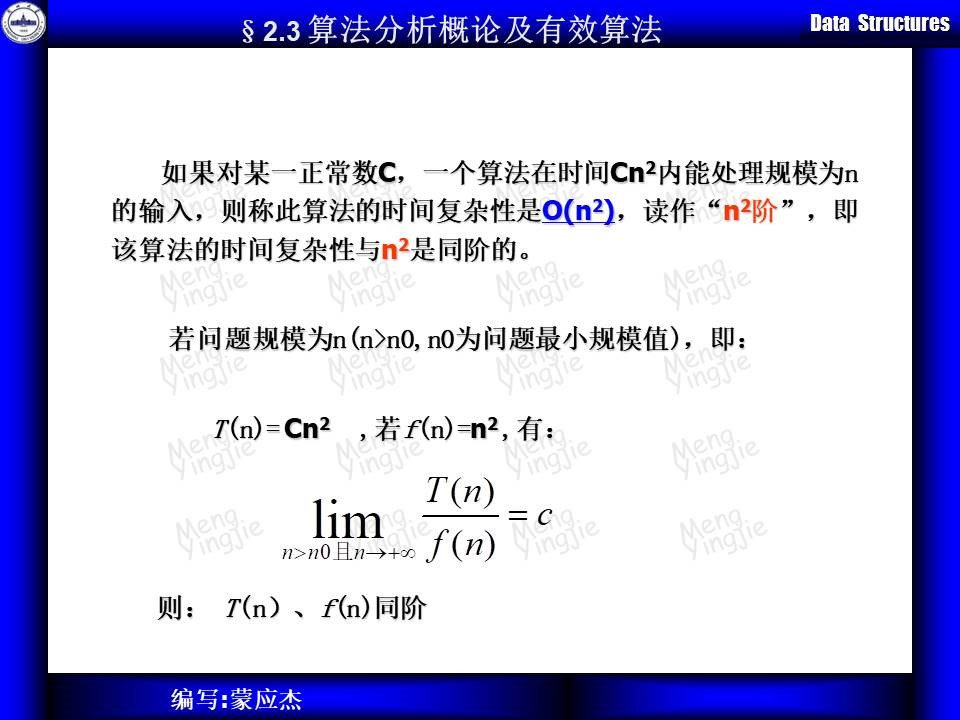
\includegraphics[width=0.7\textwidth]{figures/2.1.jpg}
			    
			    \label{fig_install_texlive}
			\end{figure}

			若一个算法时间复杂度为O(($2^{n}$),称其需要指数时间;若是O(($n^{k}$),称其为多项式时间。当n非常大时两个时间差异非常大。

			以多项式时间为界限的算法称为有效算法。如果一个问题不存在以多项式时间为界限的算法,称为难解的(难解性问题)。

			\begin{figure}[H]
			    \centering
			    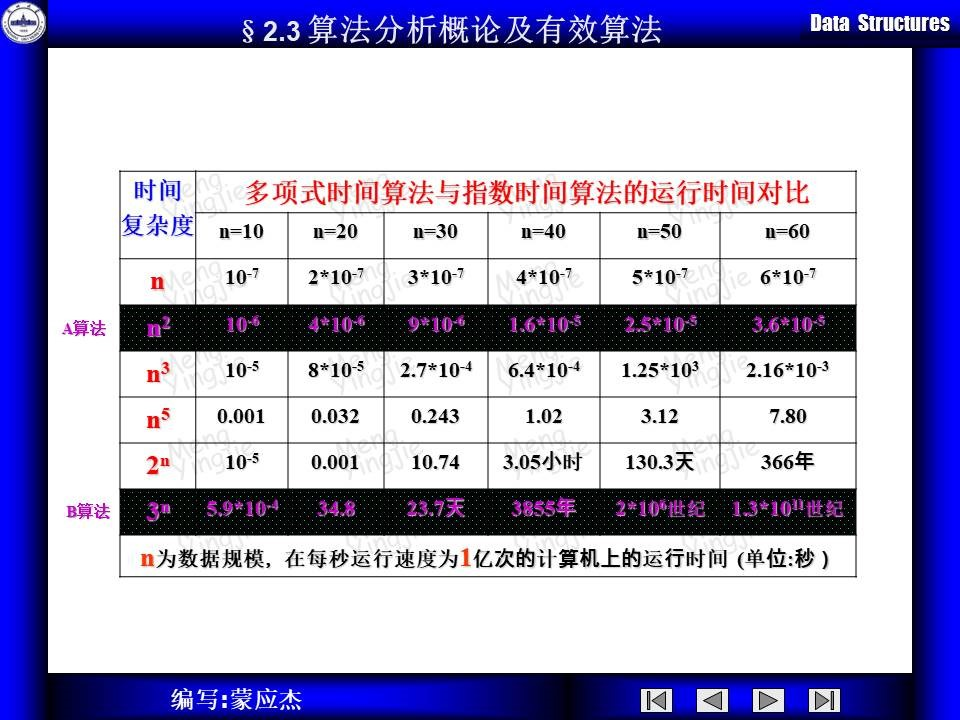
\includegraphics[width=0.7\textwidth]{figures/2.2.jpg}
			    
			    \label{fig_install_texlive}
			\end{figure}

			当n非常大时两个时间差异非常大。

			\begin{figure}[H]
			    \centering
			    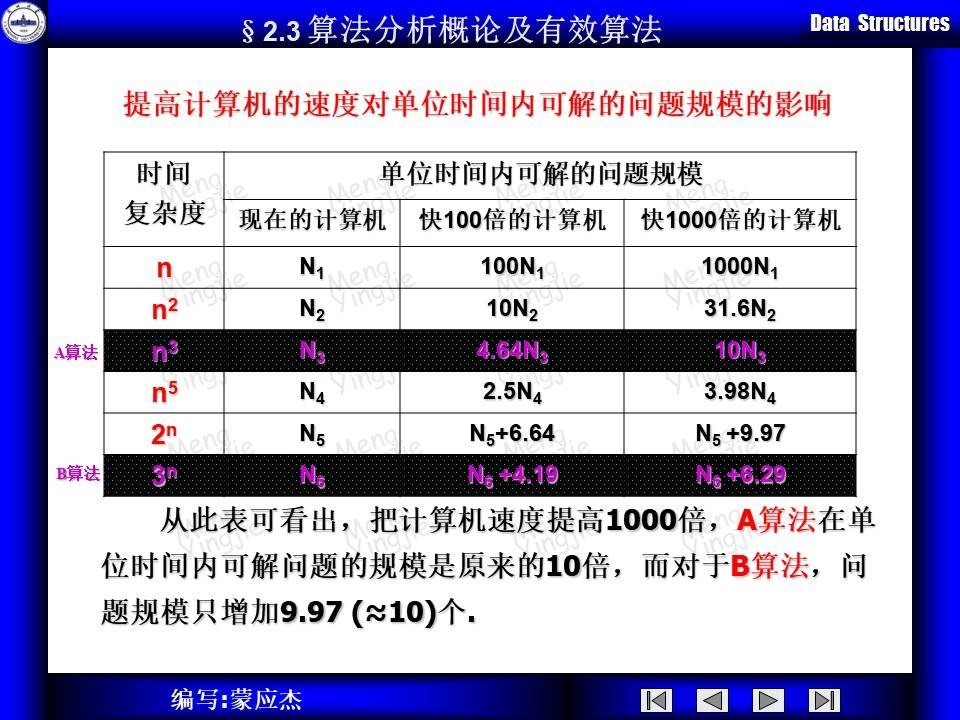
\includegraphics[width=0.7\textwidth]{figures/2.3.jpg}
			    
			    \label{fig_install_texlive}
			\end{figure}

			对于时间复杂度,会关注时间复杂度的ϱ最坏情况和时间复杂度的平均情况。

		\subsection{复杂性分析}

			不需要知道精确的数值,只需要知道他一个规模。

			\begin{itemize}
				\item 时间复杂性的分析
					\begin{enumerate}
						\item 根据问题的特点合理选择一种或几种操作作为整个算法的“标准操作”(假设循环执行次数最多,循环就是标准操作)
						\item 确定每个算法在给定输入下总共执行了多少次标准操作,并根据次数推导求出时间函数
						\item 确定该函数的阶
					\end{enumerate}
				\item 空间复杂性的分析
					\begin{enumerate}
						\item 根据问题的特点合理选择一种或几种操作作为整个算法的“标准操作”(假设循环执行次数最多,循环就是标准操作)
						\item 确定每个算法在给定输入下总共执行了多少次标准操作,并根据次数推导求出时间函数
						\item 确定该函数的阶
					\end{enumerate}
				
					要求各个算法的存储结构一样的前提下,关注算法所需的附加存储空间复杂性

			\end{itemize}

	\section{算法设计方法概论}
		\subsection{概述}
			\begin{itemize}
				\item 用科学的方法进行算法设计
				\item 最常用方法:自顶向下 逐步求精

						顶层:问题的总和、抽象全貌

						底层:问题的具体化、展开、细节

						求精的方法:

					\begin{enumerate}
						\item 分而治之

								将问题划分为一些不相交的部分,依次解决

						\item 作出有限进展

								采用一个朝解的方向得到有限进展的方法,反复应用,逐渐逼近

						\item 情况分析

								对问题各种情况给予分析,选择适当方案。

					\end{enumerate}

				\item 健壮性
				\item 高效性
			\end{itemize}

		\subsection{算法设计的基本技术}
			以下内容不做要求
			\begin{itemize}
				\item 穷举法
				\item 分治法
				\item 回溯法
				\item 分支界限法
				\item 动态规划法
				\item 贪心法
			\end{itemize}

	\section{算法描述语言}
		\subsection{PDL概述}

			Program、Design、Language

			即伪码语言,主要用来书写软件设计的规约,是基于我们自然语言与具体的成设计语言之间的一种语言。这是一种保留计算机、程序设计、语言的基本框架和描述形式,并去掉一些特异性和直接性的要求,再结合自然语言所形成的一种用于描述算法处理的逻辑语言。

		\subsection{PDL的优势}
			\begin{itemize}
				\item 表达能力强,具有关键字的固定语法。提供了特定的结构化控制结构
				\item 引入了自然语言的一些习惯,结构比较清晰,简单易读
				\item 容易转化为任何一种程序设计语言代码(可由PDL生成程序代码)
			\end{itemize}

		\subsection{PDL书写及要求}
			\begin{enumerate}
				\item 算法的框架
					\begin{itemize}
						\item 一般过程的书写框架
\begin{lstlisting}
PROC 过程名(I/O参数);
BEGIN
	语句组
END;
\end{lstlisting}
						\item 函数过程的书写框架
\begin{lstlisting}
FUNC 函数名(I/O参数):类型名;
BEGIN
	语句组
END;
\end{lstlisting}
					\end{itemize}
				\item 词的定义及说明

						标识符:按照一定的规则形成的具有特定含义的一个词。
						\begin{itemize}
							\item 过程名:调用前需定义
							\item 常量名、变量名:使用前需说明

									例如VAR i,j,k:integer

									常见的数据类型名写法及表示:
									\begin{itemize}
										\item 整数型:integer
										\item 实数型:real
										\item 布尔型:boolean
										\item 字符型(单字符):char
										\item 子介型(用于表达范围):下界..上界,例如40..90(表示40-90),'A'..'G'
										\item 枚举类型:{0,1,2,3}  元素次序不能变
										\item 构造类型
											\begin{itemize}
												\item 数组型:
\begin{lstlisting}
ARRAY[下标类型] OF 成分类型
\end{lstlisting}
												例如:
\begin{lstlisting}
A: ARRAY[1..20] OF integer
\end{lstlisting}
\begin{lstlisting}
B: ARRAY[1..20,-10..20] OF real	
//(B是点集,二维数组)
\end{lstlisting}
												\item 记录型:
\begin{lstlisting}
RECORD
	域标识符1:类型1
	              …
	域标识符n:类型n
END
\end{lstlisting}
例如:
\begin{lstlisting}
A=RECORD
	Name:ARRAY[1…8] OF char;
	Sex:0..1
	Age:interger;
  END
\end{lstlisting}

											\end{itemize}
										\item 指针类型:
\begin{lstlisting}
↑ 类型名
\end{lstlisting}
例如:
\begin{lstlisting}
TYPE A=↑integer;		//指针类型
\end{lstlisting}
\begin{lstlisting}
VAR B:↑integer;			//指针变量
\end{lstlisting}

									\end{itemize}

						\end{itemize}
				\item 基本语序
					\begin{itemize}
						\item 赋值语句:
\begin{lstlisting}
变量名←表达式
\end{lstlisting}
						\item 流程图
						\item 条件语句
							\begin{itemize}
								\item 形式一
\begin{lstlisting}
if 条件 then 语句组
\end{lstlisting}
								\item 形式二
\begin{lstlisting}
if 条件 then 语句组1
	else 语句组2
\end{lstlisting}
							\end{itemize}
						\item 循环语句
							\begin{itemize}
								\item 当型(while)
\begin{lstlisting}
WHILE 条件 DO
	语句组;
\end{lstlisting}
								\item 直到型(repeat)
\begin{lstlisting}
REPEAT
	语句组;
UNTIL 条件
\end{lstlisting}
								\item 从到型(for-to)
									\begin{itemize}
										\item 默认步长为1:
\begin{lstlisting}
FOR 变量←初值 TO 终值 DO
	语句组;
\end{lstlisting}
										\item 自定义步长:
\begin{lstlisting}
FOR 变量←初值 TO 终值 STEP 步长值 DO
	语句组;
\end{lstlisting}
										\item 倒数:
\begin{lstlisting}
FOR 变量←初值 DOWNTO 终值 DO
	语句组;
\end{lstlisting}
									\end{itemize}

							\end{itemize}
						\item 输入语句:
\begin{lstlisting}
read(变量名表);
\end{lstlisting}
例:
\begin{lstlisting}
read(x,y,z);
\end{lstlisting}
						\item 输出语句
\begin{lstlisting}
write(变量名表);
\end{lstlisting}
					\end{itemize}
				\item 拓展语序
\begin{itemize}
	\item 情况语句
\begin{lstlisting}
CASE
	条件1:语句组1;
	条件2:语句组2;
	……
	条件n:语句组n;
	[ELSE 语句组n+1]
ENDCASE
\end{lstlisting}
	\item 一般过程调用语句:
\begin{lstlisting}
Call 过程名;
\end{lstlisting}
	\item 函数过程调用:通过在表达式中引用函数名完成,即被引用函数名出现在表达式中
	\item 出错提示语句:
\begin{lstlisting}
error(错误信息);
\end{lstlisting}
	\item 终结语句
\begin{lstlisting}
Exit 	\\算法转向正常结束
\end{lstlisting}
\begin{lstlisting}
Return \\算法转向正常结束,携带值离开
\end{lstlisting}
\begin{lstlisting}
Abort 	\\中途废止(中止)
\end{lstlisting}
	\item 复合语句
\begin{lstlisting}
[ 	简单语句1;
	简单语句2;
	……
	简单语句n;	]
\end{lstlisting}
或用Begin End 代替括号

	\item 动态符号
\begin{itemize}
	\item 储存单元的引用:
\begin{lstlisting}
指针变量名↑
\end{lstlisting}
例:
\begin{lstlisting}
x↑
\end{lstlisting}
	\item 动态空间分配:
\begin{lstlisting}
New(P)
\end{lstlisting}
	\item 动态空间回收:
\begin{lstlisting}
Dispose(P)
\end{lstlisting}
	\item 空地址的表示:
\begin{lstlisting}
Nil
\end{lstlisting}
\end{itemize}
\end{itemize}
			\end{enumerate}

\chapter{线性表}
	\section{线性表及其运算}
		\subsection{线性表的定义}
		线性表的定义:一个线性表是n$\ge$0个数据元素$a_{1}, a_{2}, \dots \dots, a_{n}$的有限序列,序列中除第一及最后一个元素以外,每个元素有且只有一个直接前驱和直接后继。

		简称表,可表示为:$A=\left(a_{1}, a_{2}, \dots \dots, a_{n}\right)$
\begin{lstlisting}
ai:datatype	//表示ai 项可以是任何类型
\end{lstlisting}

		\subsection{线性表的特征}
			\begin{itemize}
				\item 有限的。线性表的表长:线性表元素的个数。控标的长度定义为0
				\item 元素呈线性关系。元素的位置只取决于他们自己的逻辑顺序。
			\end{itemize}

		\subsection{线性表的运算}
			\begin{itemize}
				\item 确定线性表的长度n

				\item 存取线性表的第i个数据元素,检验或改变某个数据项的值
				\item 在第i-1个和第i个数据元素之间插入一个新的数据元素。约定插入的元素是第i个元素的直接前驱
				\item 删除第i个元素
				\item 将两个或两个以上的线性表合并成一个线性表
				\item 将一个线性表拆分成两个或两个以上的线性表
				\item 重新复制一个线性表
				\item 对线性表中的数据元素依据某一种规则进行重组
			\end{itemize}

	\section{线性表的储存表示}
\begin{itemize}
	\item 线性表的向量表示
		\begin{itemize}
			\item 存储方法
			顺序地分配存储单元,且每个数据元素占据相同大小的存储空间(顺序且等长)

			\item 数据访问
			TODO
			\item 向量存储结构特性
				\begin{itemize}
					\item 储存分配呈线性结构
					\item 属于随机存储结构(访问一个元素的代价与元素位置无关,即访问任何一个元素(找地址)的运算量一样,一维数组,通过下标变量来访问(数组构造的本质即算公式))

				\end{itemize}
			\item 向量存储结构的形式化表示
			可用一个一维数组表示,由于数组属于静态结构,其空间规模须事先定义(1..max),要有个计数器记录数组长度(空间规模)

			表述形式:
\begin{lstlisting}
TYPE SQLIST:ARRAY[1..max] OF datatype;
## 内容
VAR n:0..max;	
## 计数器(记录数组长度)
\end{lstlisting}
\begin{lstlisting}
TYPE SQLIST= RECORD 
		data:ARRAY[1..max] OF datatype;
## 内容 n:0..max; ## 计数器(记录数组长度) 
             END;
\end{lstlisting}
			\item 插入
			\item 删除
			\item 小结
		\end{itemize}

	\item 线性表的链表表示
		\begin{itemize}
			\item 单链表表示
\begin{lstlisting}
TYPE pointer=↑node;
     node= RECORD 
		data: datatype;
		next: pointer;
           END; 
	link=pointer;
\end{lstlisting}
			\item 带表头的单链表表示
			\item 带表头结点的循环单链表表示
			\item 带表头结点的双向循环链表表示
\begin{lstlisting}
TYPE pointer=↑node;
     node= RECORD 
		Left: pointer;
		data: datatype;
			
		right: pointer;
           END;
     dblink=pointer;
\end{lstlisting}
		\end{itemize}
\begin{figure}[H]
    \centering
    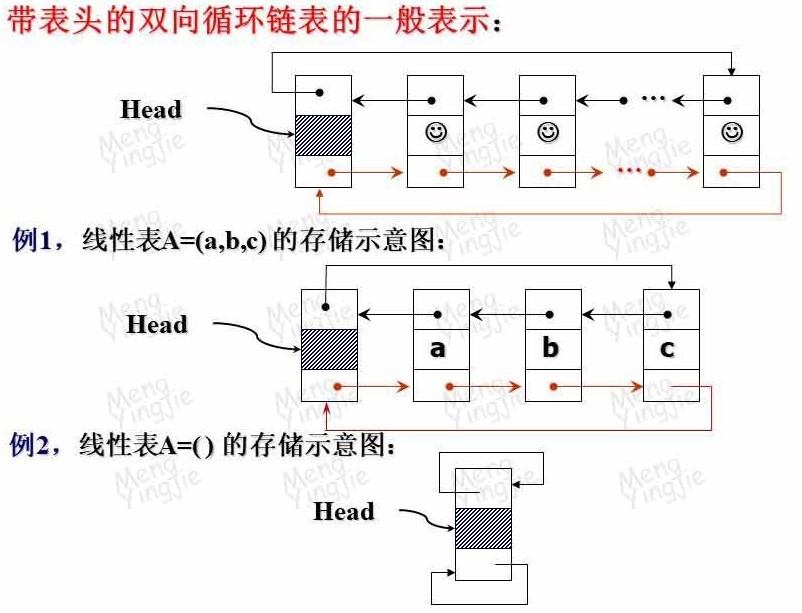
\includegraphics[width=0.7\textwidth]{3.1.jpg}
    \label{fig_install_texlive}
\end{figure}
\begin{figure}[H]
    \centering
    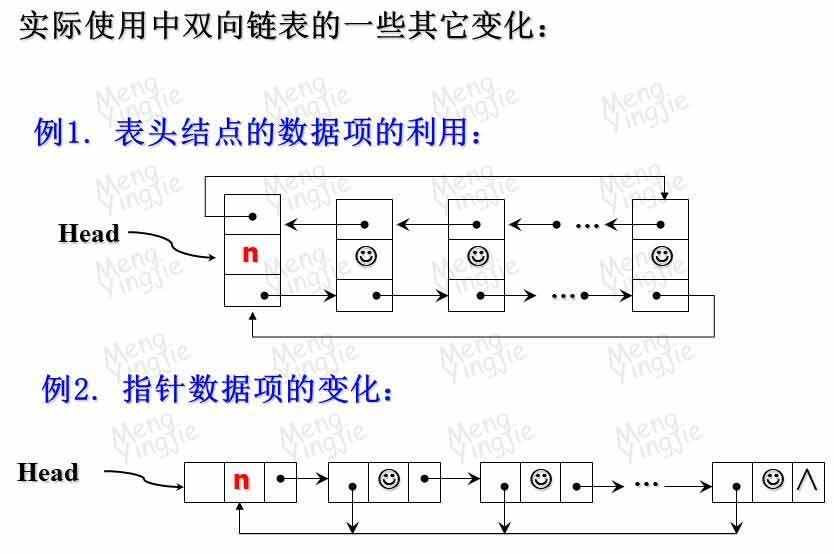
\includegraphics[width=0.7\textwidth]{3.2.jpg}
    \label{fig_install_texlive}
\end{figure}
	\item 线性表的应用
\end{itemize}


\chapter{栈和队列}
	\section{栈及其运算}
	栈是工具性数据结构。
		\subsection{绪论}
		\subsection{栈的基本定义}
		栈是一个下限为常数,上限可变化的向量(或者反之)。有时称为堆栈或堆阵。

		后进先出表(LIFO)。

		可变化一端称为栈顶,不变化的一端称为栈底。

		\subsection{与线性表的关系}
			\begin{itemize}
				\item 相同点
					\begin{itemize}
						\item 逻辑关系都是线性关系
					\end{itemize}

				\item 不同点
					\begin{itemize}
						\item 线性表可以从任意位置增删,栈的增删只能从表尾进行
						\item 栈的运算是线性表的一个子集,且这个子集还需加以约束
					\end{itemize}

			\end{itemize}

		\subsection{栈的运算}
			\begin{itemize}
				\item 入栈,PUSH(S),完成往栈中加入元素的过程,即插入操作,也称为压栈
				\item 出栈,POP(S),完成从栈中取出元素的过程,即删除操作,也称为弹出
			\end{itemize}

		\subsection{栈的存储与运算的实现}
		\subsection{多栈共存问题}

	\section{栈的应用}

	\section{队列及其运算}
		\begin{itemize}
			\item 绪论
			分时和并行,主要处理对稀缺资源的争夺
			\item 队列的定义
			队列是一个下限和上限只能增加而不能减少(下限和上限的指针只能往一个方向移动)的向量(或者反之)

			先进先出表(FIFO)
			\item 队列与线性表
			\begin{itemize}
				\item 相同点
					\begin{itemize}
						\item 逻辑关系都是线性关系
					\end{itemize}

				\item 不同点
					\begin{itemize}
						\item 线性表可以从任意位置增删,队列的只能一端插入一端删除
						\item 队列的运算是线性表的一个子集,且这个子集还需加以约束
					\end{itemize}

			\end{itemize}
			\item 队列的运算
				\begin{itemize}
					\item 出队
					\item 入队
				\end{itemize}

			\item 队列的存储与运算的实现
		\end{itemize}

	\section{受限的栈及队列(了解)}
		\begin{itemize}
			\item 双端队列

			双端队列是一种所有的插入和删除都限制在表的两端进行的线性表
			\item 双栈

			双栈是一种加限制的双端队列,即从哪端进就只能从哪端出,就像是两个底部相连的栈
			\item 超队列

			超队列是一种删除受限制的双端队列,删除限制在一端,插入可以在两端
			\item 超栈

			超栈是一种插入受限制的双端队列,插入限制在一端,删除可以在两端
		\end{itemize}

\chapter{串}
	\section{串及其运算}
	\begin{itemize}
		\item 概述
		
		字符串是线性表模型数据元素实例化的体现

		全称字符串

		早期:作为输入输出的常量和提示

		热点:中文信息处理
		\item 串的定义
		
		一个由零个或多个字符组成的有穷序列称为串

		简记为$A=^{\prime}a_{1} a_{2} a_{3} \dots a_{n}^{\prime}$

		串的长度:串中所含的字符个数

		空串:串长为零的串,记作Φ
		
		非空串

		空白串:空白字符组成的串,记作$^{\prime}\sqcup^{\prime}$

		串的相等:串长也相等,对应位置上的字符也一样

		字串/主串:一个串中任意个连续字符组成的子序列称为该串的子串,该串成为它的所有子串的主串。不一定是一个真子集
		\item 串的运算
			\begin{itemize}
				\item 赋值
				
				assign(S,chars)  将字符串常量chars赋给字符串变量S
				\item 连接
			
				concatenation(S,T) 将字符串S和T联接在一起
				\item 取子串
			
				substring(S,m,n) 从第m个位置开始取n个连续字符(通常)/从第m个位置开始到第n个位置
				\item 求子串序号
		
				strindex(S,T,i) 确定串T在S中第一次出现的位置i
				\item 串的插入
			
				strinsert(S,T,i)
				\item 串的删除
			
				strdelete(S,m,n)
				\item 串的复制
		
				copy(S,T)
				\item 串的置换
				
				replace(A,B,C)(找到A中的B用C来替换)

				replace(S,m,n,T)(把S字符串的(m到n/从m开始的n个字符)用T来替换)
			\end{itemize}
		\item 串的存储
			\begin{itemize}
				\item 顺序储存

				一般用向量来表示,通常称为字符串数组、字符串变量、字符串常量
					\begin{itemize}
						\item 压缩模式

						按字节存储数据 (C语言)

						\item 非压缩格式

						运算器以字为单位运算,存储器以字节为单位,为了避免转换浪费的时间,存储器以字为单位存储一个字符,变成非压缩模式(只存一个字母需要一个字的空间,比较浪费)
					\end{itemize}
				\item 索引储存

				多用在对于多个字符串常量或者变量的组织
				\item 链接储存

				理论上研究的多,实际上用的少,不易于实现
			\end{itemize}
	\end{itemize}

	\section{串的模式匹配}
		\begin{itemize}
			\item 概述

	在模式分类或者问题回答系统等方面,将输入模式与样本模式进行匹配的过程啊,我们就把它称为模式匹配。
	
	通常把S称为目标(或正文),把P称为模式,把从目标S中查找模式P的过程称为模式匹配。
	
	串的匹配是模式匹配的实例化。

			\item 匹配的朴素算法(Brute-Force算法)
			\begin{figure}[H]
			    \centering
			    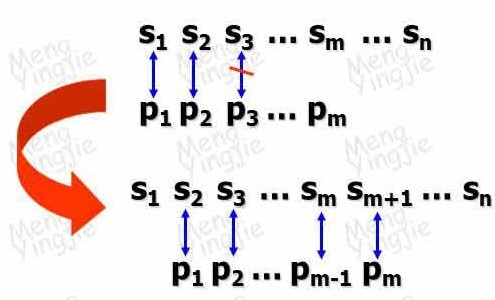
\includegraphics[width=0.7\textwidth]{figures/5.1.jpg}
			    
			    \label{fig_install_texlive}
			\end{figure}

			处理基本思想:对正文顺序搜索
				\begin{enumerate}
					\item 逐次比较(对应字符依次比较)
					\item 发现不匹配时,将P相对于S右移一位
					\item 重复上述过程,直到成功或扫描完S
				\end{enumerate}
			\begin{figure}[H]
			    \centering
			    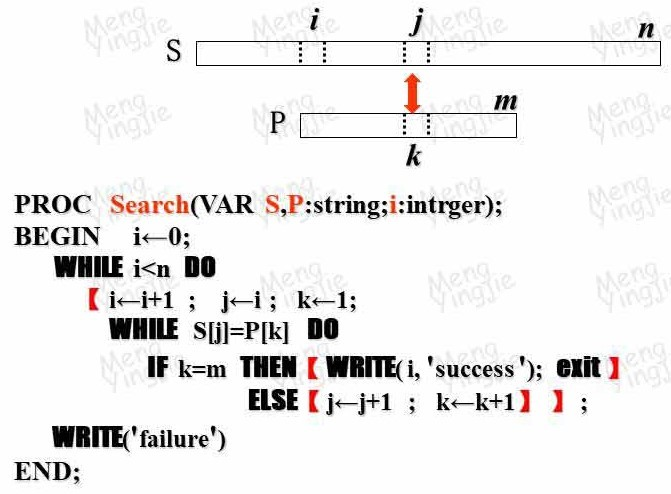
\includegraphics[width=0.7\textwidth]{figures/5.2.jpg}
			    
			    \label{fig_install_texlive}
			\end{figure}

			优化算法:KMP算法
		\end{itemize}

	\section{例题}
	2019年兰州大学开源社区纳新面试题中有一题关于字符串的运算,现将我的解决方案附于后文。

给出一个文本文件,其中每个单词不包括空格及跨行,单词由字符序列构成且不区分大小写,完成以下功能:统计给定单词在文本文件中出现的总次数。

注:允许使用 string.h

\begin{lstlisting}[language=c]
#include<stdio.h>
#include<string.h>

char word[100];
char text[10000];
int count = 0;

char trans(char c){
    if(c >= 'A'&&c <= 'Z'){
        c = c + 'a' - 'A';
    }
    return c;
}

void getword() {
    char c;
    int i = 1;
    while (1) {
        c = getchar();
        if (c == '\n') break;
        word[i] = trans(c);
        i++;
    }
    word[0] = i - 1;//第0位存放单词长度
    return;
}

void gettext() {
    char c;
    int i = 1;
    while (1) {
        c = getchar();
        if (c == EOF) break;
        text[i] = trans(c);
        i++;
    }
    text[0] = i - 1;//第0位存放文本长度
    return;
}

void check() {

    int i = 0, j = 0;
    int flag = 1;
    while (1) {
        i++;
        j++;
        if (i == text[0]) break;
        if (text[i] == '\n' || text[i] == ' ') {
            j = 0;
            flag = 1;
            continue;
        }
        if (flag == 0) {
            continue;
        }
        if (text[i] != word[j])
            flag = 0;
        if (j == word[0]) {
            if (flag == 1) {
                if (text[i + 1] == '\n' || text[i + 1] == ' ')
                    count++;
            }
            flag = 1;
        }
    }
}

int main()
{
    freopen("C:\\Users\\Kente\\Desktop\\123\\text.txt", "r", stdin);//假设给出的文本文件第一排是给定单词,第二排及之后是要统计的文本
    getword();
    gettext();
    check();
    printf("%d", count);
    return 0;
}

/*text.txt
ABC
Abc abC dasasdsa abc
dasdasdasdasd dasdasdasdasd
abc ab
*/
\end{lstlisting}

\chapter{数组和广义表}
	\section{数组的定义与运算}
		\subsection{定义}

一维数组是一个向量,它的每个元素是该结构中不可分割的最小单位;n(n>1)维数组是个向量,它的每个元素是n-1维数组,且具有相同的下限和上限。

向量(只有量值而无方向的量)是标量的一维的有序集合。
		\subsection{运算}
\begin{itemize}
	\item 给定一组下标,存取相应数据元素
	\item 给定一组下标,修改相应的数据元素的某个属性的值
\end{itemize}
	\section{数组元素的地址访问}
		\subsection{概述}
	数组是一种静态存储结构,数组定义需给出数组规模。数组元素访问依靠下标变量。

	词典编辑序:
\begin{itemize}
	\item 行主序(行优先,行为主)(更常见)

从上到下,每行从左到右
	\item 列主序

从左到右,每列从上到下
\end{itemize}
\begin{figure}[H]
    \centering
    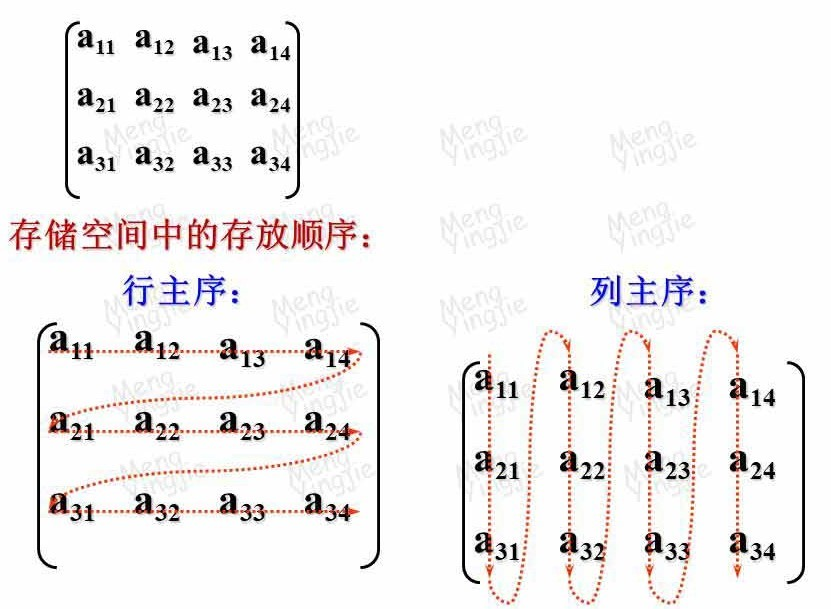
\includegraphics[width=0.7\textwidth]{6.1.jpg}
    \label{fig_install_texlive}
\end{figure}


		\subsection{地址计算}
(默认讨论行主序)
			\subsubsection{二维数组}
设置数组$A\left(c_{1}, . d_{1}, c_{2} \dots d_{2}\right)$,首地址为$\operatorname{Loc}\left(c_{1}, c_{2}\right)=A O(A)$(基地址),元素长度为l
\begin{figure}[H]
    \centering
    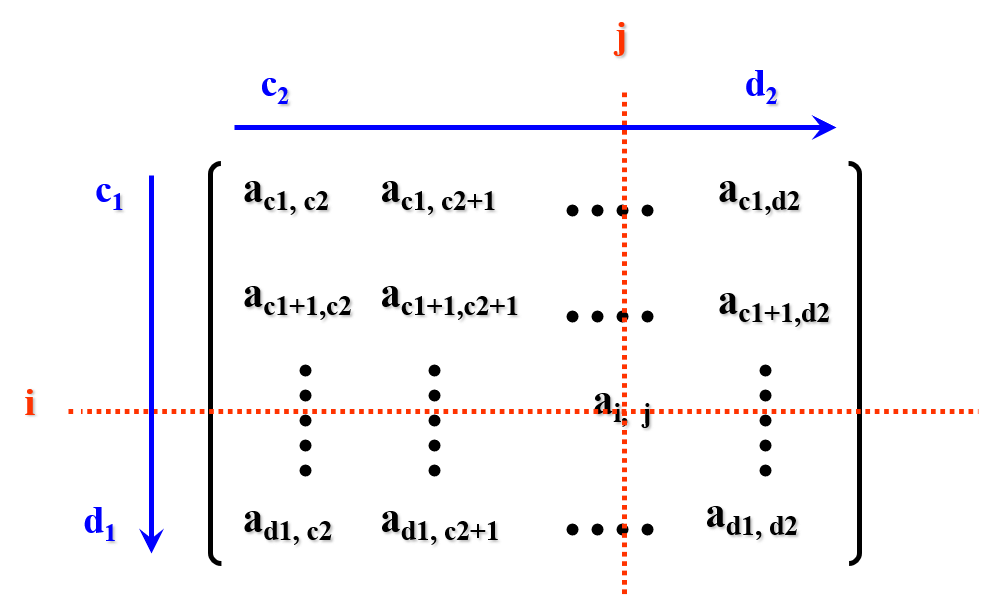
\includegraphics[width=0.7\textwidth]{6.2.png}
    \label{fig_install_texlive}
\end{figure}
$\operatorname{Loc}(i, j)=\left[\left(i-c_{1}\right)\left(d_{2}-c_{2}+1\right)+\left(j-c_{2}\right)\right]^{*} l+A O(A)$

二维数组是随机存储结构。
			\subsubsection{多维数组}
设置数组$A\left(c_{1} \ldots d_{1}, c_{2} \ldots d_{2}, \ldots, c_{n} \ldots d_{n}\right)$,首地址为$\operatorname{Loc}\left(c_{1}, c_{2}, c_{3}, \dots, c_{n}\right)=A O(A)$(基地址),元素长度为l。
\begin{figure}[H]
    \centering
    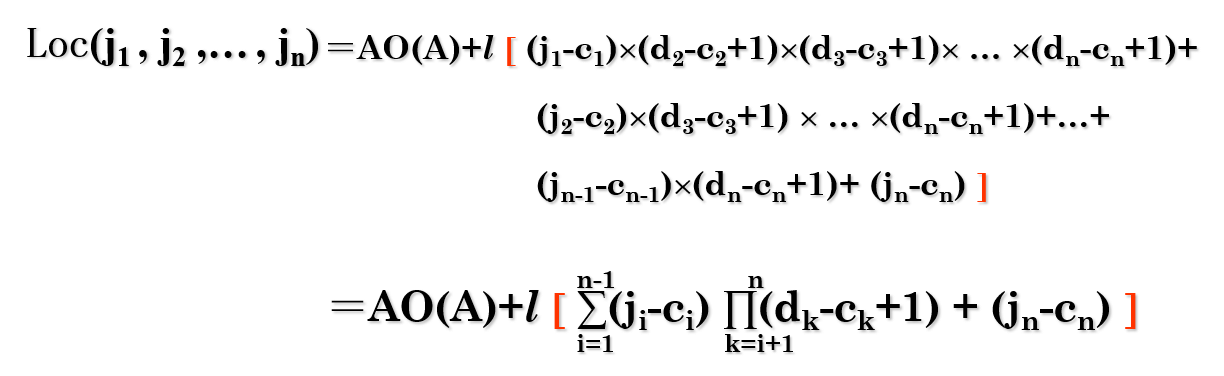
\includegraphics[width=0.7\textwidth]{6.3.png}
    \label{fig_install_texlive}
\end{figure}
\begin{figure}[H]
    \centering
    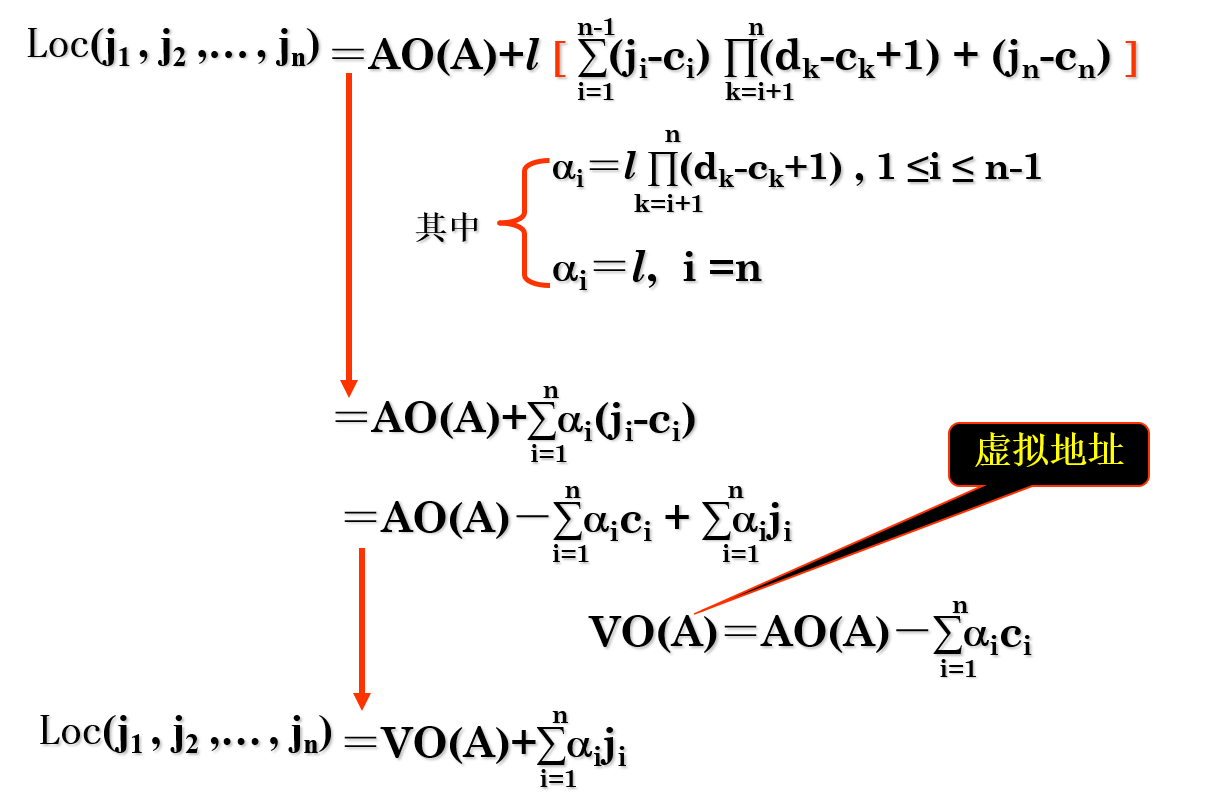
\includegraphics[width=0.7\textwidth]{6.4.png}
    \label{fig_install_texlive}
\end{figure}
			多维数组是随机存储结构。

			数组编译就是利用公式把虚拟地址运算出来。

地址访问公式中的常数项之和就是虚拟地址。
		\subsection{特殊数组}
			\subsubsection{三角矩阵}
\begin{figure}[H]
    \centering
    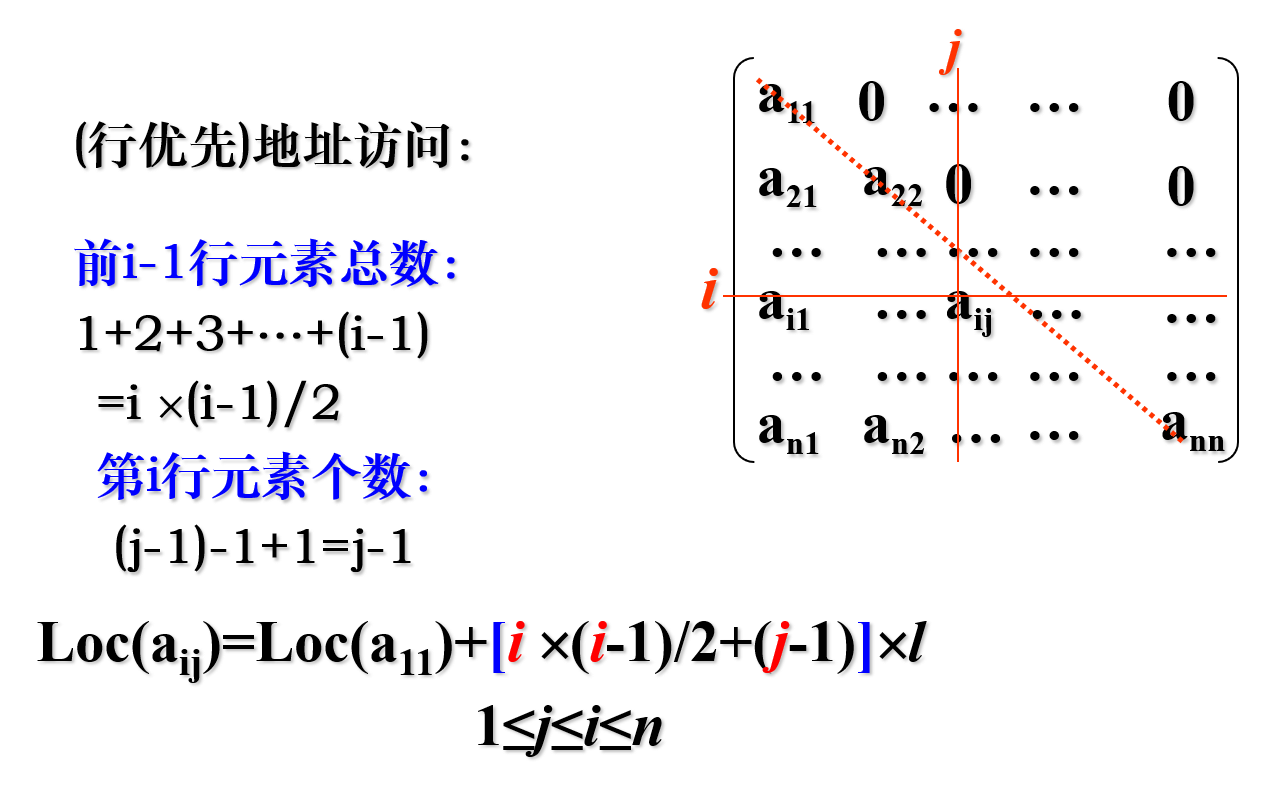
\includegraphics[width=0.7\textwidth]{6.5.png}
    \label{fig_install_texlive}
\end{figure}
			\subsubsection{三对角矩阵}
\begin{figure}[H]
    \centering
    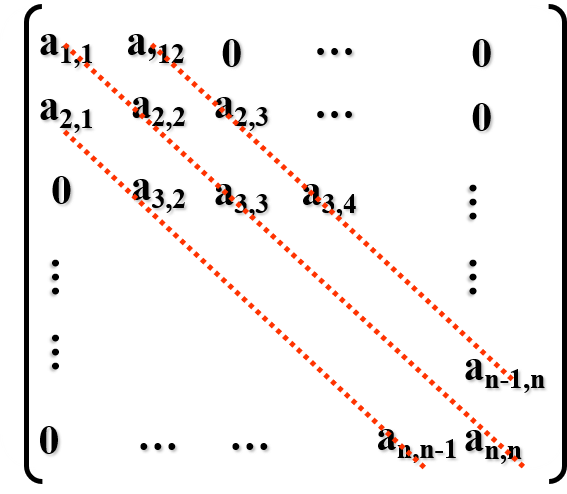
\includegraphics[width=0.7\textwidth]{6.6.png}
    \label{fig_install_texlive}
\end{figure}


	\section{稀疏矩阵}
		\subsection{概要}
研究重点:研究特殊存储方法。
		\subsection{定义}
			\subsubsection{稀疏数组}
在一个数组当中和某元素比较而言,不相同的元素很少时,我们称此数组为稀疏数组。
		
“某元素”指的是大量的雷同元素,可以认为是0。
		
“很少”指的是远远小于。

			\subsubsection{稀疏矩阵}
在一个矩阵当中和某元素比较而言,不相同的元素很少时,我们称此矩阵为稀疏矩阵。
			\subsubsection{特殊矩阵与稀疏矩阵的异同}
特殊矩阵的雷同元素分布有规律,稀疏矩阵的雷同元素分布无规律。

		\subsection{稀疏矩阵的存储}
按照行(或列)优先的原则 ,将矩阵中的非零元素顺序存放,为便于检索和存取,一般须带有适当的辅助信息。
			\subsubsection{顺序存储}
\begin{itemize}
	\item 三元组(triad)表示
		\begin{itemize}
			\item 两种实现方式
				\begin{itemize}
					\item 视为一维的记录数组
\begin{figure}[H]
    \centering
    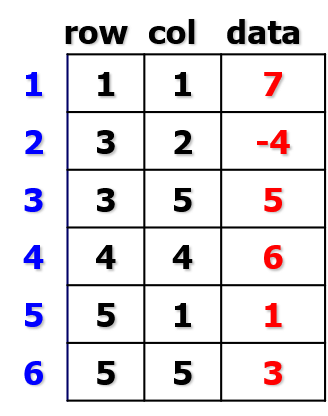
\includegraphics[width=0.7\textwidth]{6.7.png}
    \label{fig_install_texlive}
\end{figure}
					\item 视为二维数组
\begin{figure}[H]
    \centering
    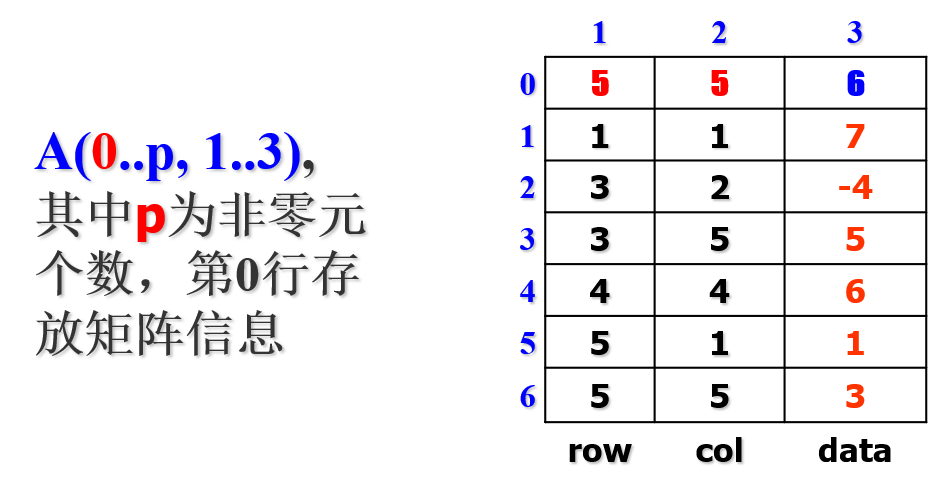
\includegraphics[width=0.7\textwidth]{6.8.png}
    \label{fig_install_texlive}
\end{figure}
				\end{itemize}
			\item 缺陷
				\begin{itemize}
					\item 用向量实现,属于静态结构
					\item 元素规模事先确定
					\item 插入删除运算才会带来大规模的元素的移动
				\end{itemize}

		\end{itemize}

	\item 索引表示(二元组表示)

三元组中数据元素按row呈有序状态(行优先次序决定),故可建立行索引表,即标记每行的非零元起始位置
\begin{figure}[H]
    \centering
    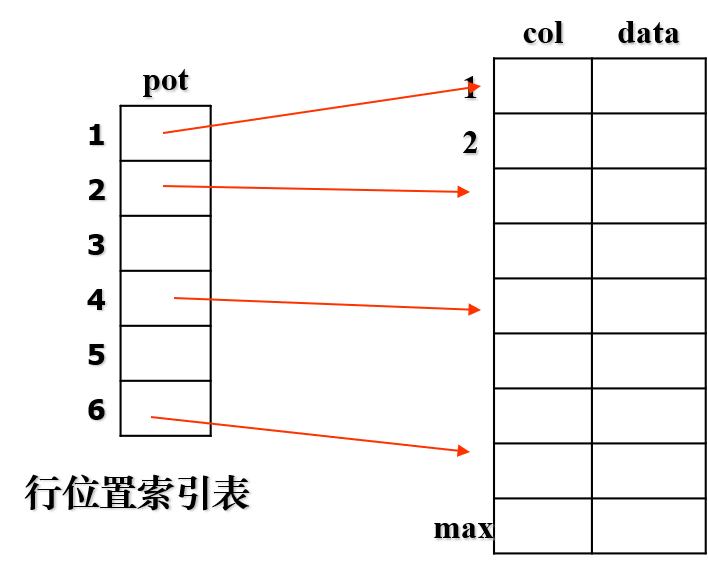
\includegraphics[width=0.7\textwidth]{6.9.png}
    \label{fig_install_texlive}
\end{figure}
	\item 伪地址表示

按照非零元在矩阵中出现的相对次序作为元素的地址映射关系来组织元素次序(在行或列优先的次序下)。
			
缺陷:计算之前先要用一下原有数组那个编译器当中那个计算公式计算它是第几个

\end{itemize}
			\subsubsection{链接存储}
				\begin{itemize}
					\item 单链表
					\item 十字链表

对于非零元素依据行、列特性,每一行和每一列建立一个循环链表。
\begin{figure}[H]
    \centering
    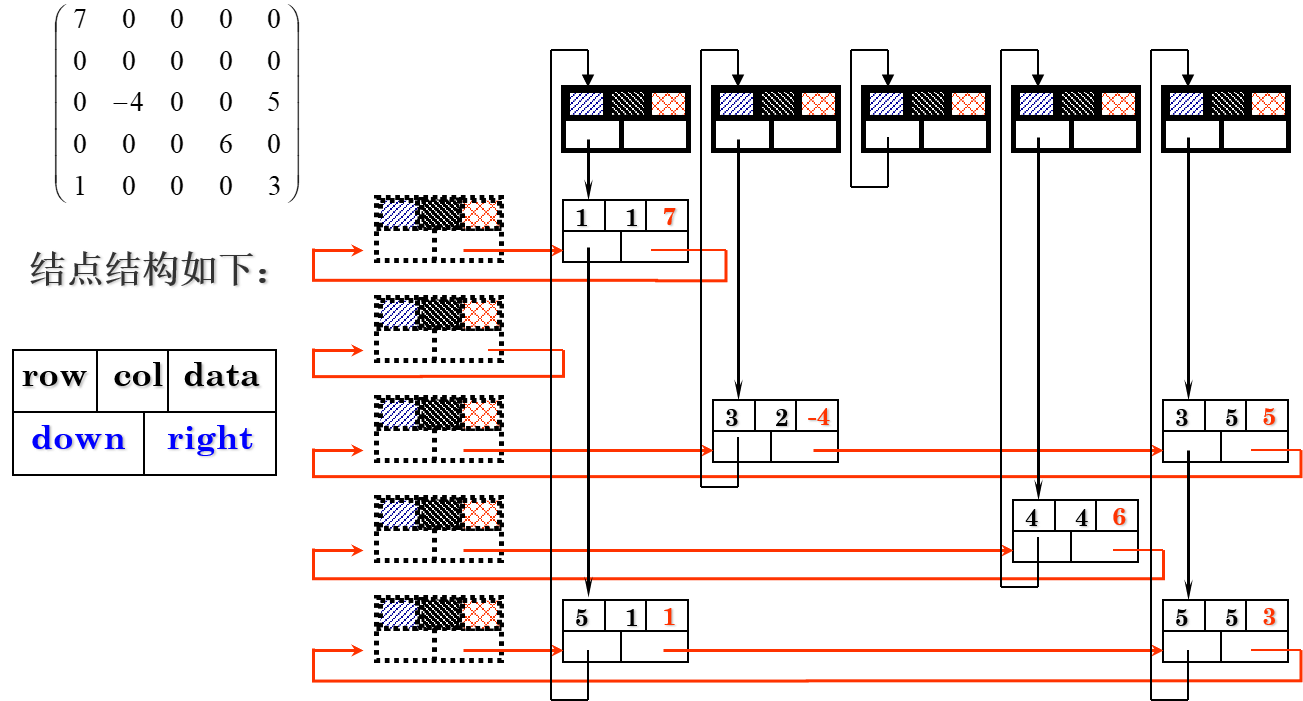
\includegraphics[width=0.7\textwidth]{6.10.png}
    \label{fig_install_texlive}
\end{figure}
行表头(虚线)向下域没用处;列表头(实线)向右域没用处;行列表头节点可以共享。
表头结点的数据项是没有用的。用表头结点的数据把所有的表头结点串起来。此时数据项称为共享(C中的共用体)。
				\end{itemize}

			\subsubsection{散列存储}
		\subsection{稀疏矩阵的运算}
保持结构的一致性。
	\section{广义表(了解)}
		\subsection{定义}
			\subsubsection{自然语言:}
广义表是零个或多个原子或子表所组成的有限序列。一般简称为列表或表。

			\subsubsection{形式化表示为:$A=\left(a_{1}, a_{2}, \dots, a_{i}, \dots, a_{n}\right)$}
组成一个表的元素$a_{i}$可以是原子(即数据元素),也可以是子表。

原子是数据元素,是我们要处理的真实的客观事物,是一个确定的概念。
		
子表是作为构成元素的表,这是一个递归定义。

			\subsubsection{广义表的表长:}
表包含的元素的个数。要素可以是原子数据,也可以是子表。

长度为0的表为空表。
			\subsubsection{广义表的深度:}
出现的表中套表这种嵌套的层次数目的最大值。

大写字母表示集合、一堆数据;小写字母表示具体客观事物。
\begin{figure}[H]
    \centering
    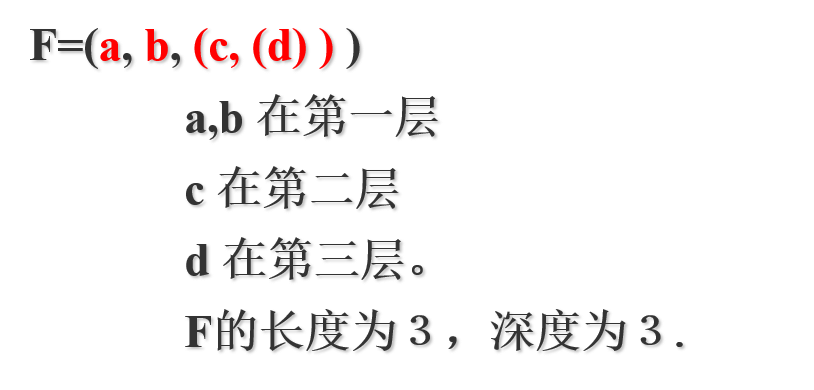
\includegraphics[width=0.7\textwidth]{6.11.png}
    \label{fig_install_texlive}
\end{figure}
举例:
\begin{figure}[H]
    \centering
    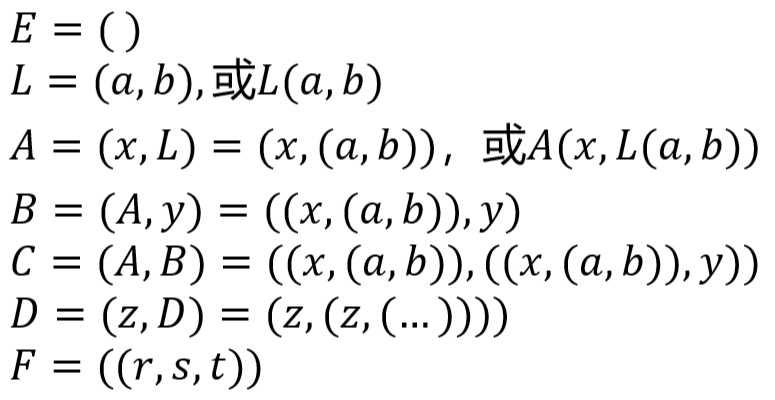
\includegraphics[width=0.7\textwidth]{6.12.png}
    \label{fig_install_texlive}
\end{figure}
		\subsection{特性}
			\subsubsection{定义是递归的}
			\subsubsection{定义没有限制元素的共享性和递归性}
\begin{itemize}
	\item 共享性:组成要素可以是任何现存的已经存在的表
	\item 递归性:广义表可用自身作为元素使用(可能导致问题)
\end{itemize}

		\subsection{存储}
			\subsubsection{顺序存储方式}
			\subsubsection{链接存储方式}
\begin{itemize}
	\item 等长模式
	\item 非等长模式
\end{itemize}

\chapter{树形结构}
	\section{树的基本定义和运算}
		\subsection{树形结构的概述}
			\begin{itemize}
				\item 与线性结构的差异
				
				直接后继可以是多个
				\item 树形结构的地位

				树是计算机中最重要的非线性结构
				\item 讨论内容
					\begin{itemize}
						\item 逻辑角度
						\item 存储方式
						\item 应用
						\item 模型
						\begin{itemize}
							\item 树
							\item 二叉树
						\end{itemize}
					
					\end{itemize}

			\end{itemize}

		\subsection{树的基本定义}
		树T,是满足如下性质的有限个节点组成的非空集合
			\begin{itemize}
				\item T中有且仅有一个称为根的结点
				\item 除根结点之外,其余结点分成m(m>0)个不相交的集合T1,T2,…,Tm,其中每个Ti 都是树,而且都称为T的子树。
			
			\end{itemize}
		注意
\begin{itemize}
	\item 是递归定义
	\item 定义中对于子树的个数及次序没有进行任何约束
	\item 与图论中的树不同,是有向图中的根树的特例。隐含了向下的方向性

\end{itemize}

		\subsection{有序树的基本定义}
		在树T中如果子树T1,T2,..,Tn 的相对次序是重要的(即有序的),则称T为有向有序树,简称有序树。

		默认树是有序树


\begin{figure}[H]
    \centering
    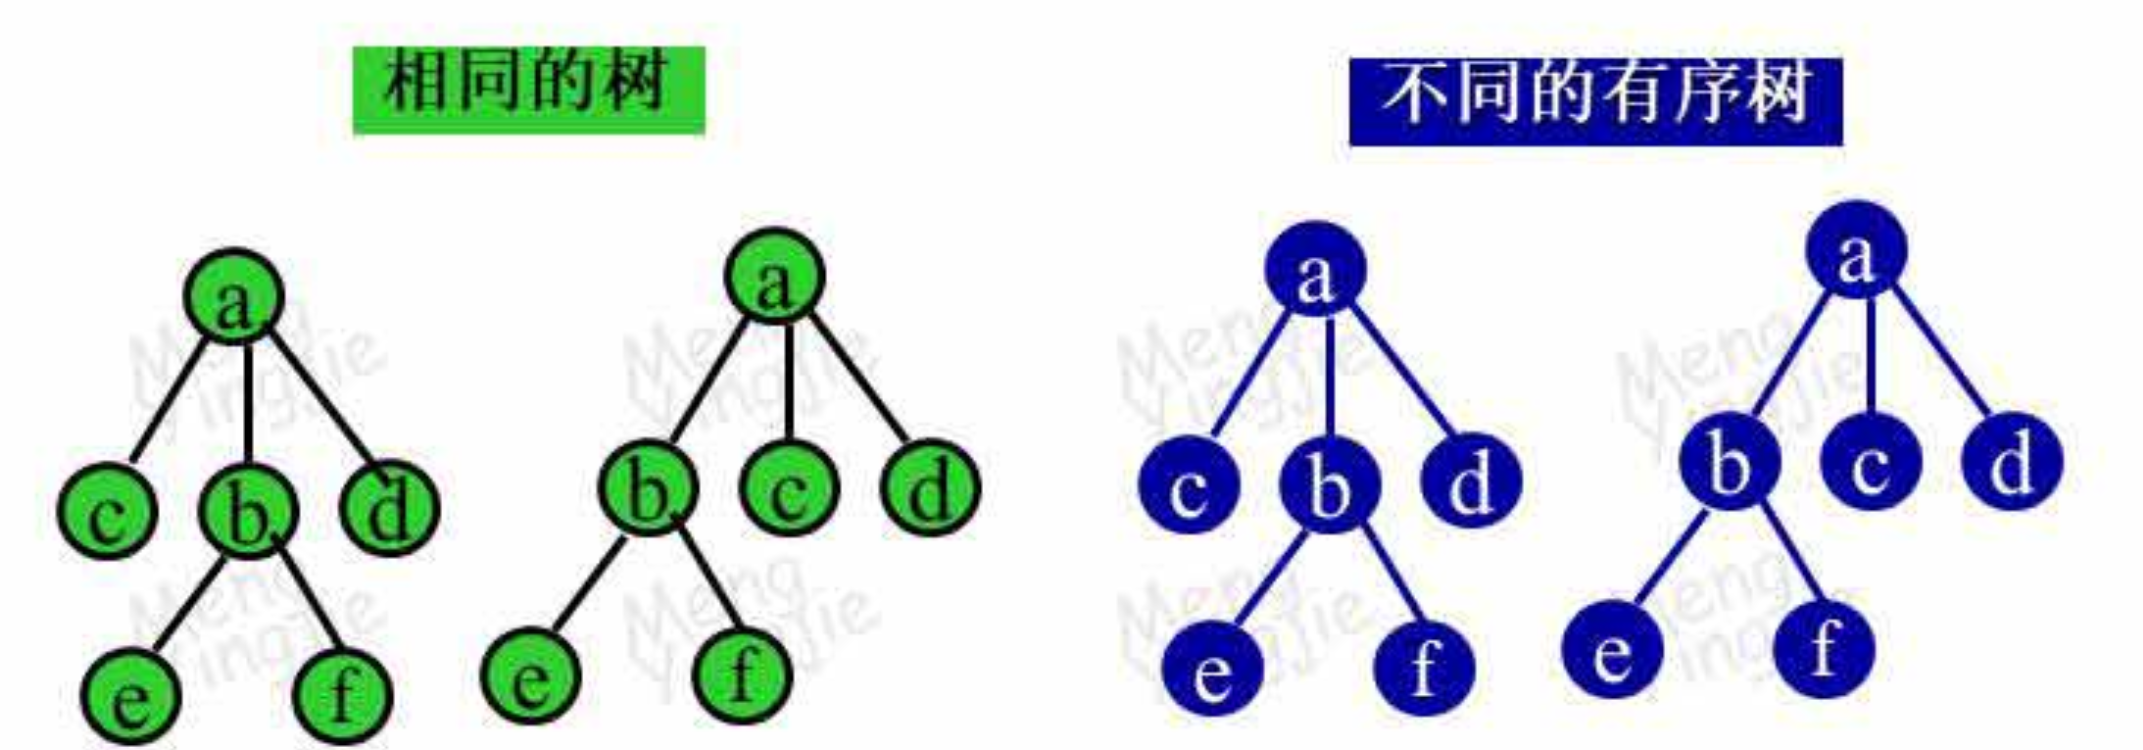
\includegraphics[width=0.7\textwidth]{figures/7.1.png}

\end{figure}

		\subsection{森林(树林)}
		森林是零棵或多棵不相交的树的集合(通常是有序集合)

	\section{二叉树}
		\begin{itemize}
			\item 定义
			\item 特性
			\item 二叉树的存储表示
		\end{itemize}

	\section{遍历二叉树}
		\subsection{概念}
		定义:对于给定的数据结构,系统地访问该结构中的每个结点,且每个结点仅被访问一次的操作过程称遍历

		系统地:按照一定的规律、次序

		访问:对元素进行的某种操作

		遍历本质上是一个运算过程(序列)

		对于给定的二叉树,系统地访问该结构中的每个结点,且每个结点仅被访问一次的操作过程称遍历

		\subsection{二叉树的遍历次序(order)}
			\begin{itemize}
				\item 层次策略
					\begin{itemize}
						\item 自上而下
							\begin{enumerate}
								\item 从左到右
								\item 从右到左
							\end{enumerate}
						\item 自下而上
					\end{itemize}
				\item 深度策略
				遍历针对结构,是一个过程;访问针对一个点,是一个动作。
				\begin{figure}[H]
				    \centering
				    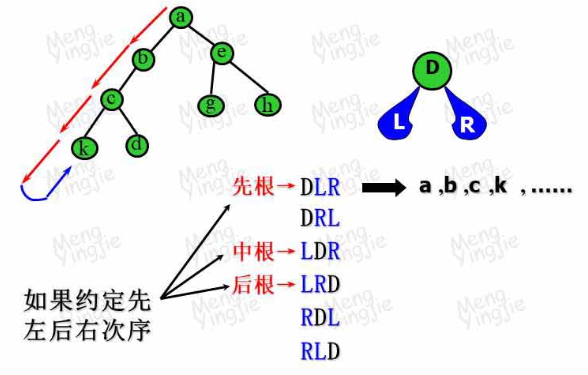
\includegraphics[width=0.7\textwidth]{figures/7.2.png}
				    
				    \label{fig_install_texlive}
				\end{figure}
				\begin{itemize}
					\item 先根(前序)DLR

					先拿到根,然后从左子树走,又是二叉树,则访问了左子树的根节点,再往下走,直到访问到k,左子树为空,回到c,访问右子树。沿着纵深往下搜索,只要有子树就往下搜索,先不管兄弟。
					\item 中根LDR
					\item 后根(后序)LRD
				\end{itemize}

			\end{itemize}

	\section{树、森林与二叉树的转换}
		\subsection{概述}
		转换原因
		\begin{itemize}
			\item 二叉树有许多优良特性,而树没有
			\item n叉树中二叉树的空间利用率最高
		\end{itemize}
		\subsection{树转为二叉树}
		这里约定树为有序树,子树的次序相对固定

		转换规则:
		\begin{enumerate}
			\item 加线(亲兄弟之间加上虚连线)
			\item 抹线(除了最左子节点之外,抹掉所有节点与其余子节点的连线)
			\item 调整(调成二叉树的样子,原有连线在左,新加连线在右)
		\end{enumerate}
		\begin{figure}[H]
		    \centering
		    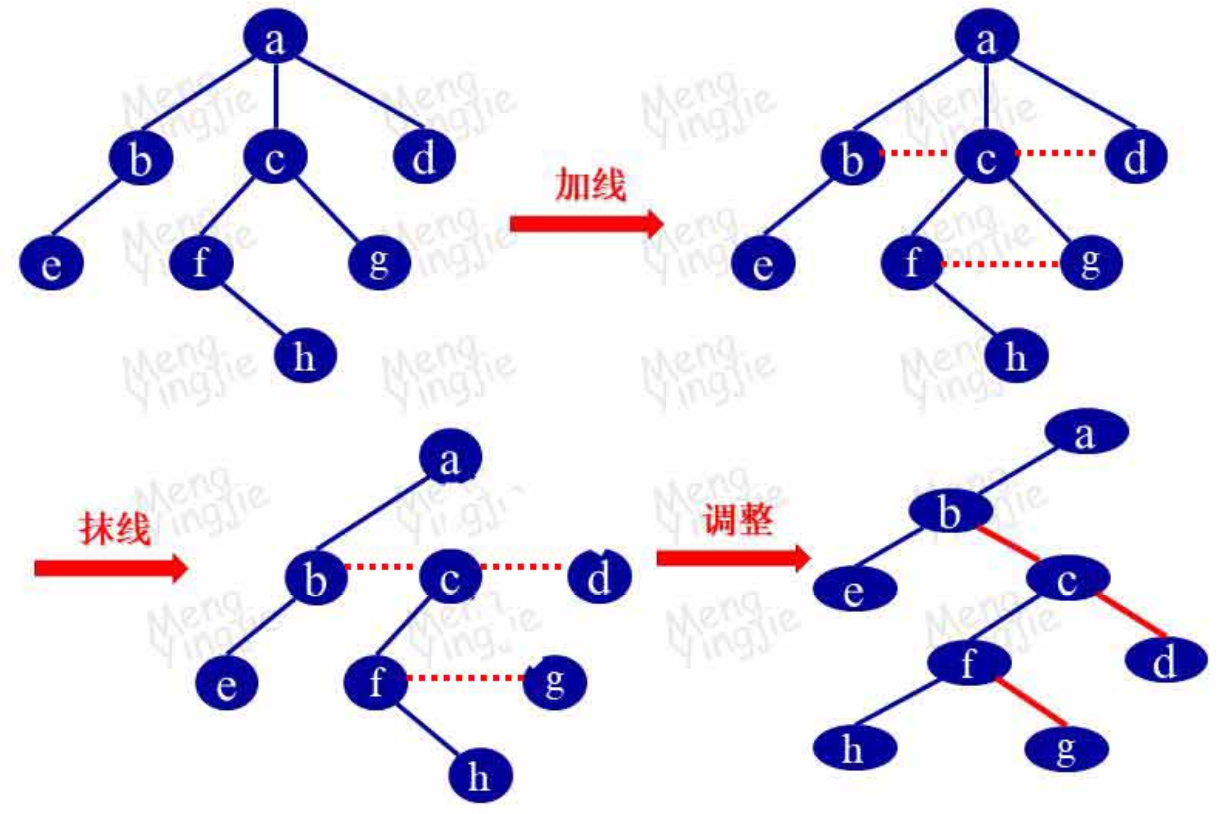
\includegraphics[width=0.7\textwidth]{figures/7.3.png}
		    
		    \label{fig_install_texlive}
		\end{figure}
		特点:
		\begin{itemize}
			\item 原有兄弟成为右结点及右结点的右列结点
			\item 根子树仅有左节点
		\end{itemize}

		\subsection{二叉树还原为树}
		转换规则:
		\begin{enumerate}
			\item 加线(如果有个节点X是父结点的左子树,那么它的右子树,右子树的右子树...都与X的父节点加线)
			\item 抹线(所有节点抹掉与右子树的连线)
			\item 调整(让节点按层次分布)
		\end{enumerate}

		\subsection{森林转为二叉树}
		两种方法:
		\begin{itemize}
			\item 方法一:树转换

			将每棵树转为二叉树
			\item 方法二:二叉树连接
		
			依据转换得到的二叉树的次序,将后一棵作为前一棵根节点的右子树,因为树转二叉树的根节点无右子树
			\begin{figure}[H]
			    \centering
			    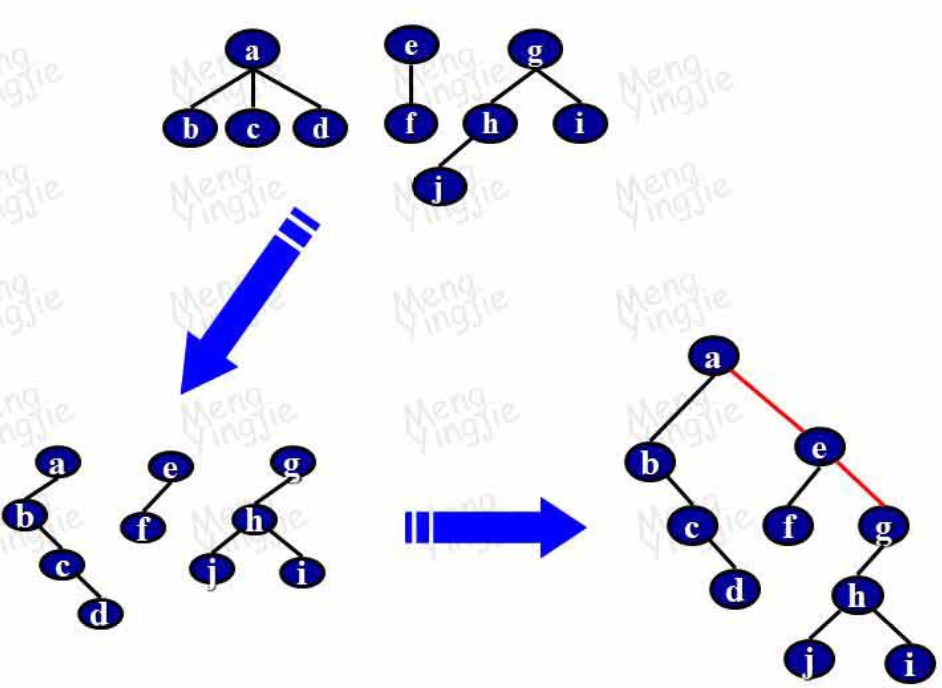
\includegraphics[width=0.7\textwidth]{figures/7.4.png}
			    
			    \label{fig_install_texlive}
			\end{figure}
		\end{itemize}

		\subsection{二叉树转为森林}
		转换规则:
		\begin{enumerate}
			\item 抹线(沿着根节点,抹掉其右子树与根节点的连线,不断往右下搜索)
			\item 还原(把每棵二叉树还原树)
		\end{enumerate}
		\begin{figure}[H]
		    \centering
		    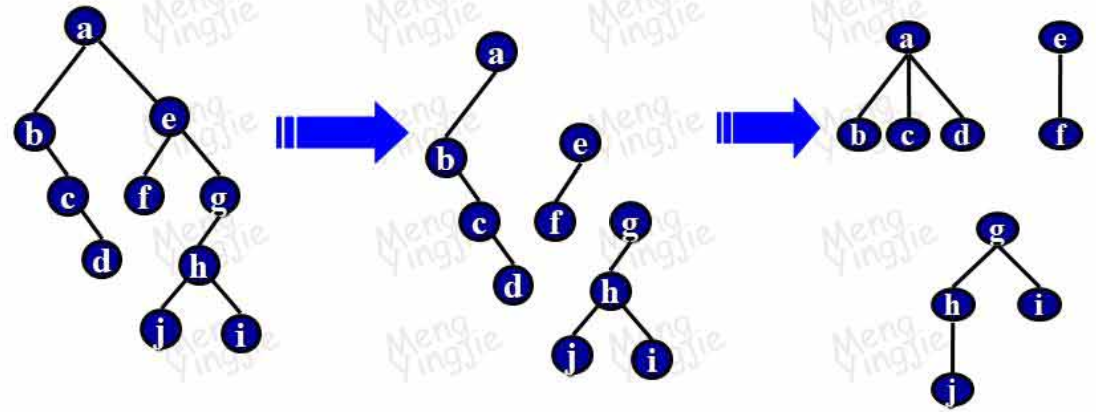
\includegraphics[width=0.7\textwidth]{figures/7.5.png}
		    
		    \label{fig_install_texlive}
		\end{figure}

		\subsection{树的遍历}
		\begin{itemize}
			\item 方法一:树转换

			将每棵树转为二叉树后再处理,处理完成后还原
			\item 方法二:直接处理

						遍历次序
						\begin{itemize}
							\item 层次策略
								\begin{itemize}
									\item 自上而下
										\begin{enumerate}
											\item 从左到右
											\item 从右到左
										\end{enumerate}
									\item 自下而上
								\end{itemize}
							\item 深度策略
								\begin{itemize}
									\item 先根(前序)DLR
										\begin{enumerate}
											\item 访问树的根节点
											\item 先根次序下依次遍历树的根节点的每个子树
										\end{enumerate}
									\item 中根LDR
									
										一般不讨论
									\item 后根(后序)LRD
										\begin{enumerate}
											\item 后根次序下依次遍历树的根节点的每个子树
											\item 访问树的根节点
										\end{enumerate}
								\end{itemize}
						\end{itemize}
		\end{itemize}

		\subsection{森林的遍历}
		\begin{itemize}
			\item 方法一:树转换

			将每棵树转为二叉树后再处理,处理完成后还原
			\item 方法二:直接处理

					遍历次序
						\begin{itemize}
							\item 层次策略
								\begin{itemize}
									\item 自上而下
										\begin{enumerate}
											\item 从左到右
											\item 从右到左
										\end{enumerate}
									\item 自下而上
								\end{itemize}
							\item 深度策略
								\begin{itemize}
									\item 先根(前序)DLR
										\begin{enumerate}
											\item 访问第一颗树的根节点
											\item 先根次序下依次遍历第一颗树的根节点的每个子树
											\item 先根次序下依次遍历其余的树
										\end{enumerate}
									\item 中根LDR
										
									一般不讨论
									\item 后根(后序)LRD
										\begin{enumerate}
											\item 后根次序下依次遍历第一棵树的根节点的每个子树
											\item 访问第一颗树的根节点
											\item 后根次序下依次遍历其余的树
										\end{enumerate}
								\end{itemize}
						\end{itemize}
		\end{itemize}



	\section{线索树}
	\section{树形结构的应用}

\chapter{图结构}
	\section{基本概念}
		\subsection{概述}
			\subsubsection{与线性结构和树形结构的差异}
				\begin{itemize}
					\item 一个元素可以有多个直接前驱和后继
					\item 是多对多的数据关系
				\end{itemize}
			\subsubsection{地位}
		
				图结构非常重要的非线性结构。
			\subsubsection{讨论内容}
				\begin{itemize}
					\item 计算机中的图的表示方法
					\item 图的遍历
					\item 求生成树
					\item 找最短路径
					\item 拓扑排序
					\item 求关键路径
				\end{itemize}
		\subsection{概念}
			\subsubsection{图}
由n (n$\ge$1)个结点$\left\{v_{1}, v_{2}, \dots, v_{\mathrm{n}}\right\}$构成的数据G称为图,若结点集$\mathrm{V}=\left\{v_{1}, v_{2}, \dots, v_{\mathrm{n}}\right\}$上定义的称为后继的关系E是非自反的。

可表示为G=(V,E),V称为顶点集,E称为边集。只相当于

研究的图相当于离散数学中的简单图,相当于简单图,即不包含重边和环(自回路),不研究:
				
				\begin{itemize}
					\item 带自身环的图
					\item 多重图
				\end{itemize}
			\subsubsection{有向图}

在图G中,若每个关系都是顶点的有序对,则称G为有向图。

有相图的表示有两种方法:
\begin{itemize}
	\item 形式化(符号)表示

用有向线段指明了次序(方向)。
	\item 图形描述

一般用尖括弧表示顶点的有序对。
\end{itemize}
\begin{figure}[H]
	\centering
	\subfloat[形式化(符号)表示]{
        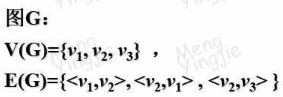
\includegraphics[width=0.4\textwidth]{figures/8.1.png}
    }\qquad
	\subfloat[图形描述]{
        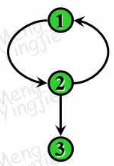
\includegraphics[width=0.4\textwidth]{figures/8.2.png}
    }\\
    \caption{图的表示方法}
    \label{fig_ide}
\end{figure}

在有向图中,若<$v_{i}$,$v_{j}$>$\in$E(G)
\begin{figure}[H]
    \centering
    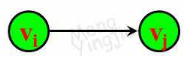
\includegraphics[width=0.7\textwidth]{figures/8.3.png}

\end{figure}
则称$v_{i}$是边的始点(或尾); $v_{j}$是边的终点(或头); 并称$v_{i}$邻接到$v_{j}$ ,$v_{j}$是从$v_{i}$邻接过来的; 称边<$v_{i}$,$v_{j}$>关联(或依附)于顶点$v_{i}$和$v_{j}$.

推论:在n个结点的有向图中,其最大边数为n(n-1)。把等于n(n-1)条边的图称有向完全图。

			\subsubsection{无向图}
在图G中,如果每个关系都是顶点的无序对,则称G为无向图。
有相图的表示有两种方法:
	\begin{itemize}
		\item 形式化(符号)表示
	
	用无向线段表示(方向)。
		\item 图形描述
	
	一般用圆括弧表示顶点的无序对
	\end{itemize}

在无向图中,若($v_{i}$,$v_{j}$)$\in$E(G)
\begin{figure}[H]
    \centering
    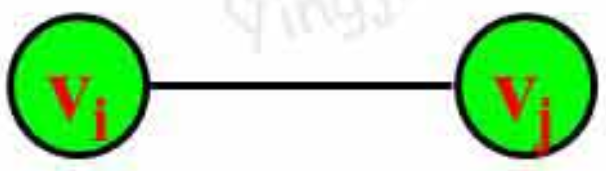
\includegraphics[width=0.7\textwidth]{figures/8.4.png}

\end{figure}
则称$v_{i}$和$v_{j}$是邻接的; 并称边($v_{i}$,$v_{j}$)关联(或依附)于顶点$v_{i}$和$v_{j}$.

在无向图中($v_{1}$,$v_{2}$)和($v_{2}$,$v_{1}$)这两个结点偶对表示同一条边。

推论:在n个结点的无向图中,其最大边数为n(n-1)/2。把等于n(n-1)/2条边的图称无向完全图。

			\subsubsection{顶点的度、入度、出度}
在图中,顶点的度(degree), 就是与该顶点关联的边的数目。

若G为无向图,则度为无向图中与某元素有关的元素的数量。

若G为有向图,则
\begin{itemize}
	\item 把以$v_{i}$为终点(头)的边的数目称作$v_{i}$的入度(incoming degree ,in-degree)(即指向该元素的边数)
	\item 把以$v_{i}$为始点(尾)的边的数目称作$v_{i}$的出度(out going degree )(即从该元素指出去的边数)
\end{itemize}

在有向图中,出度为0的顶点称终端顶点(叶子)。

推论:设图G有n个结点,t条边,若di为顶点$v_{i}$的度,显然有:TODO



			\subsubsection{子图}
设图G=(V,E), 如果有图G'=(V',E') , 且E'包含于E, V'包含于V,则称G'为G的子图。

如果图G的子图包含G的所有顶点,则该子图称为G的生成子图。

自己可以是自己的子图v。

			\subsubsection{路径、回路、图根}
对于图G=(V,E),若存在结点序列$v_{p}$,$v_{i1}$ ,$v_{i2}$ ,…,$v_{im}$, $v_{q}$使得($v_{p}$ ,$v_{i1}$),($v_{i1}$ ,$v_{i2}$),…,($v_{im}$ ,$v_{q}$)都在E(G)中(对于有向图使得<$v_{p}$ ,$v_{i1}$>,<$v_{i1}$ ,$v_{i2}$>,…,<$v_{im}$ ,$v_{q}$>都在E(G)中), 则称从顶点$v_{p}$到$v_{q}$存在一条路径(或通路,path) ,路径长度定义为这条路径上边的数目。 (路径:一个特定的点边交替序列)。

vp到vq的路径可以简写为:$v_{p}$,$v_{i}$1 ,$v_{i}$2 ,…,$v_{i}$m, $v_{q}$(用结点序简写)。

如果一条路径上的顶点除$v_{p}$和$v_{q}$可以相同以外其它顶点都不相同,则此路径为一简单路径。(即中间没有重复经过的点)。

把$v_{q}$=$v_{q}$的简单路径,称作回路(或环,loop)。(不包含自身环)。

若在一个有向图中存在一个顶点$v_{0}$,从此顶点有路径可以到达图中其它所有顶点,则此有向图称为是有根的图,$v_{0}$称作图根。(树是有向图中的有根图的特殊情况)

			\subsubsection{连通性}
\begin{itemize}
	\item 无向图

两个顶点的连通:在无向图G中,顶点u和v(u≠v)之间存在一条路径,则称顶点u和顶点v是连通的。

图的连通:对于无向图G中的任意两个顶点u,v(u≠v)都是连通的则称此无向图是连通的,或称G为连通图。(仅有无向图才谈 图的连通)。

最大(或极大)连通子图:无向图的连通分量。连通分量是一个(或多个)子图,不是一个数字。
	\item 有向图

两个顶点的连通:在有向图G中,顶点u和v(u≠v)之间存在一条从u到v和v到u的(有向)路径,则称顶点u和顶点v是连通的。(就是两个点能互相到达)

图的强连通:有向图G中的任意两个顶点u,v(u≠v)都是连通的则称此有向图是强连通的,或称G为强连通图。

一个有向图的强连通分量定义为该图的最大(或极大)强连通子图(的个数)。(有向图不谈图的连通,只谈图的强/弱连通)
\end{itemize}

			\subsubsection{网}
给图的每一条边加一个(非负的)数,这个与图的边相关的数值称为权(weight)。带权的图称为网。
带权的连通图称为网络。(网络针对无向图)

	\section{图的存储}			
		\subsection{邻接矩阵}
定义:表示顶点之间邻接关系的矩阵称邻接矩阵
			\subsubsection{图非网时}
用 boolean 矩阵表示

设图有n$\ge$1个顶点,则图G的邻接矩阵定义为n阶方阵M,M满足下列性质:
\begin{figure}[H]
    \centering
    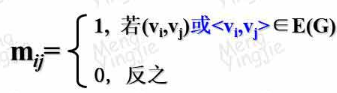
\includegraphics[width=0.7\textwidth]{8.5.png}

\end{figure}
对于无向图,它的邻接矩阵一定是一个对称矩阵,且矩阵第i行之和是顶点$v_{i}$的度

对于有向图,它的邻接矩阵一定是一个非对称矩阵,矩阵第i行之和是顶点$v_{i}$的出度,矩阵第i列之和是顶点$v_{i}$的入度。
			\subsubsection{网的邻接矩阵}
把原来的存1改成存权值。

设图有n$\ge$1个顶点,则图G的邻接矩阵定义为n阶方阵M,M满足下列性质:

\begin{figure}[H]
    \centering
    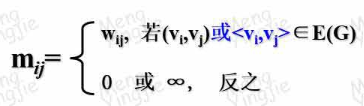
\includegraphics[width=0.7\textwidth]{8.6.png}

\end{figure}

在计算机中,∞可以取一个相对于问题而言相对大的数即可代表∞。
		\subsection{邻接表}
对图的每个顶点建立一个链表,也称邻接链表表示。

有n个结点时有n个链表,第i个链表中的结点:
			\begin{itemize}
				\item 在无向图中:是与$v_{i}$邻接的所有结点的收集。
				\item 在有向图中:是以$v_{i}$为始点的所有终点的收集。
			\end{itemize}

			\subsubsection{无向图}
\begin{figure}[H]
    \centering
    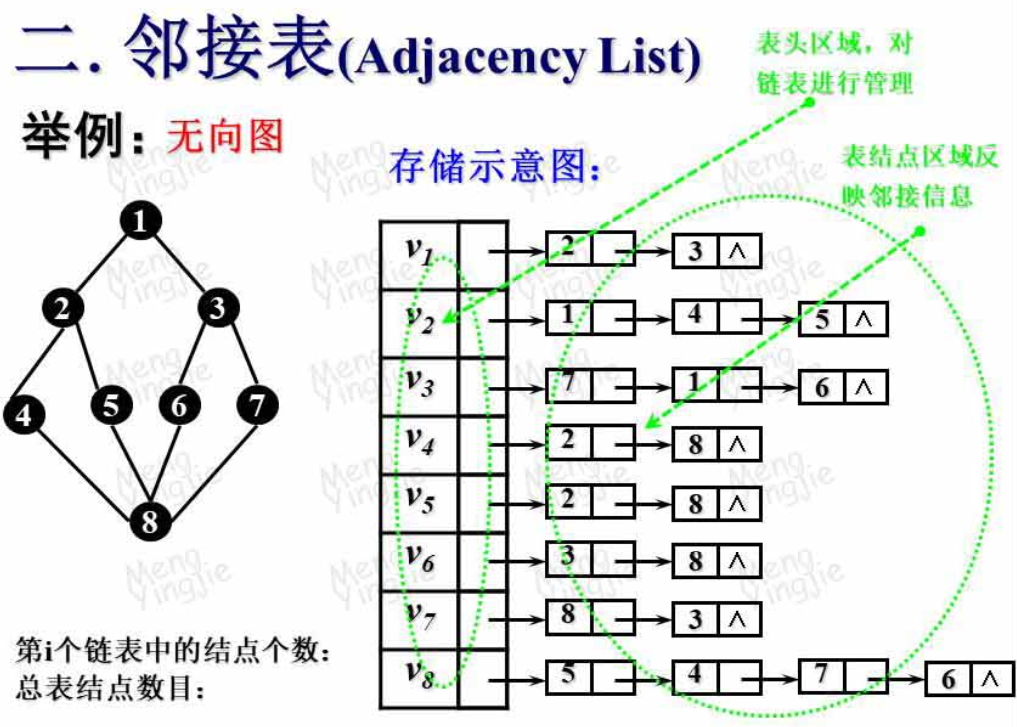
\includegraphics[width=0.7\textwidth]{8.7.png}

\end{figure}
开头的结点是线性结构,可以用向量或者链表存,此处用向量存开头的节点。

总链表结点数目:2e(每条边出现了两次)

加上表头,存储空间需n+2e

第i个链表中的结点个数: $v_{i}$的度。

无向图的邻接表,链表中的顺序可以随意变换,不分先后(即同一个图也可以有不同的邻接表)

结点间是否有边判别比邻接矩阵困难。
			\subsubsection{有向图}
\begin{figure}[H]
    \centering
    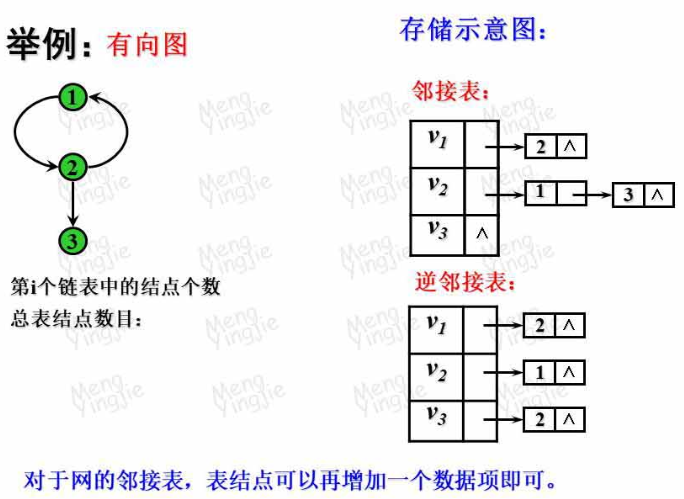
\includegraphics[width=0.7\textwidth]{8.8.png}

\end{figure}
表节点数目:e

总空间:n+e

第i个链表中的结点个数: $v_{i}$的出度。

逆邻接表:以$v_{i}$为终点的所有始点的收集。可用于获取邻接过来的结点。
		\subsection{邻接多重表}
邻接多重表以边为存储单位。

边(u, v)结点结构:
\begin{figure}[H]
    \centering
    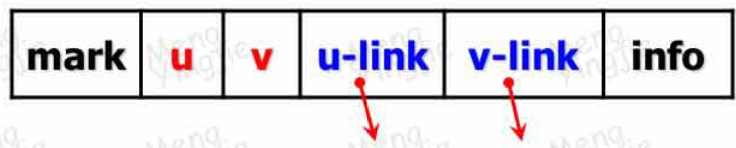
\includegraphics[width=0.7\textwidth]{8.9.png}

\end{figure}
\begin{itemize}
	\item mark:标志域,标记该边是否被处理,也可存放权值等信息
	\item u,v:关联边的两个顶点域
	\item ulink:下一条与依附于u的边的地址(指针)
	\item $v_{i}$ink:下一条与依附于v的边的地址(指针)
	\item info:其他信息
\end{itemize}


	\section{图的遍历}
		\subsection{概述}
			\subsubsection{定义}
给出图G和其中的任意一个顶点$v_{0}$(人为给出),从$v_{0}$出发系统地访问G中所有的顶点,且每个顶点仅被访问一次,这一过程称为图的遍历(graph traversal),或遍历图。
			\subsubsection{辅助结构}
须设立辅助结构,可用数组$v_{i}$sited[1..n]表征
\begin{figure}[H]
    \centering
    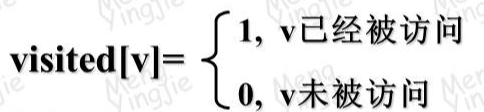
\includegraphics[width=0.7\textwidth]{8.10.png}

\end{figure}
			\subsubsection{搜索策略}
\begin{itemize}
	\item 深度优先搜索(DFS, depth-first search)

搜索中,结点扩展的次序向某一个分支纵深推进,到底后再回溯。
	\item 广度优先搜索(BFS, breadth-first search)

搜索中,对所在层次的所有结点逐个依次进行扩展后,再推进到下一个层次进行扩展。
\end{itemize}

		\subsection{图的深度优先遍历}
			\subsubsection{图的深度优先遍历的基本思想}
			\begin{enumerate}
				\item 访问出发节点 $v_{0}$,标记 $v_{0}$ 为已访问
				\item 选择一个 $v_{0}$ 邻接到的且未被访问过的结点 u
				\item 从u开始进行深搜(递归开始)
			\end{enumerate}
			\subsubsection{基于邻接表}
			面授部分讲解

		\subsection{图的广度优先遍历}
			\subsubsection{图的广度优先遍历的基本思想}
			\begin{enumerate}
				\item 访问出发点$v_{0}$
				\item 访问$v_{0}$邻接到的所有未被访问过的节点$v_{1}$,$v_{2}$,...,vt
				\item 再依次访问$v_{1}$,$v_{2}$,...,vt邻接到的所有未被访问的结点
				\item 如此进行下去,直到无法找到未被访问的结点时,则本次搜索就算结束
			\end{enumerate}
	\section{连通性及最小生成树}
		\subsection{连通分量和生成树}
			\subsubsection{求图的连通分量}
			思想:将图的遍历中搜索算法DFS(或BFS)中的访问动作具体化(即输出顶点及与之关联的边),每启动一次DFS(或BFS)就可以得到1个连通分量。
			\subsubsection{求生成树}
通过图的遍历可获取其生成子图。

对于连通图来说该生成子图,实际上是一棵树结构(恰好有n-1条边,它们把n个事物关联起来,可称其是原图的极小连通子图)

以下三种情况:
\begin{itemize}
	\item 图是连通的
	\item 图是强连通的
	\item 出发点$v_{0}$为图根
\end{itemize}
在遍历过程中,访问的节点和经过的边,所构成的生成子图,恰好可以构成一个树形结构,称为生成树。对于有n个顶点的连通图,其生成树具有n-1条边,即生成树是图的最小结构。

对于不连通的无向图和不是强连通的有向图,从任一结点出发只能得到生成森林。

生成树因为出发点不同,深、广不同而不唯一。

基于遍历方法我们可以构造极小连通子图(一谈连通图一定是无向图)(即节点不变,关联关系最小)。

			\subsection{最小生成树}
最小生成树是边的权值之和最小的网络的生成树
				\subsubsection{普里姆(Prim)算法}
				基本思想:设V={1,2,…,n}是图G的顶点集合,PRIM算法由一个初值为{$v_{0}$}的集合U开始,它每次生成一条边,逐渐长成一棵具有最小代价的生成树。

算法在每一步中都找出一个最小权的边(u,v),其中u$\in$U, v $\in$V-U.(U,V是点集,U是已经找到的点的集合,V是所有点)

即从任意一个点出发找到已找到的点集到未找到的点集中权值最小的一条路径不断连接即可

$v_{0}$:种子节点,可任选
\begin{figure}[H]
    \centering
    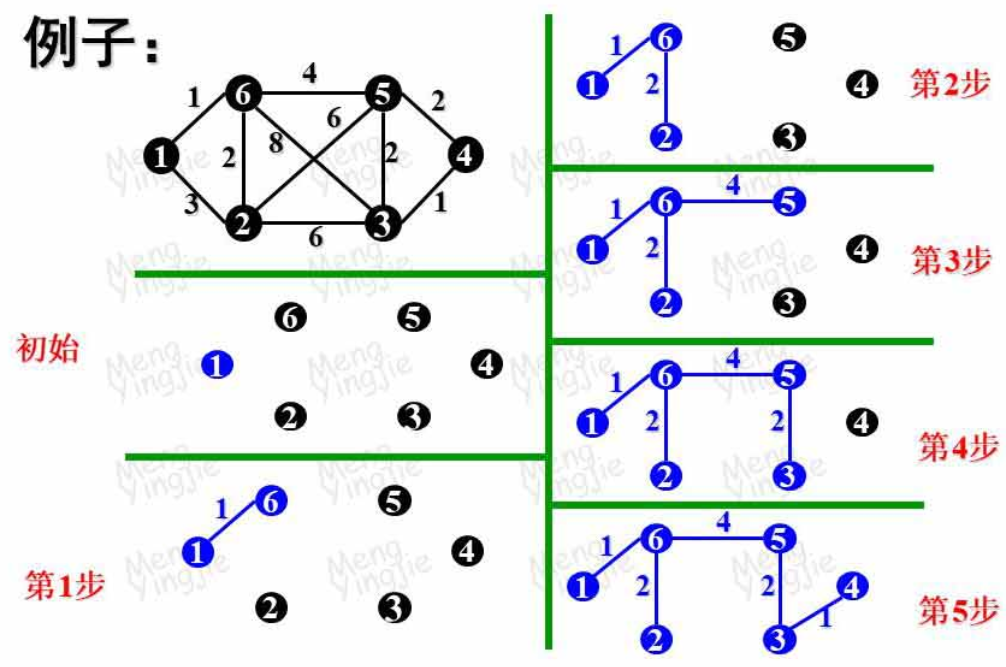
\includegraphics[width=0.7\textwidth]{8.11.png}
    \caption{普里姆(Prim)算法例子}
    \label{fig_install_texlive}
\end{figure}

				\subsubsection{克鲁斯卡尔(Kruskal)算法}
基本思想:对于图G=(V,E),该算法初始化从T=(V, Ø)开始,此时生成树是由n个连通分量(即n个孤立顶点组成)组成的一个制图——目标使得n个连通分量逐渐成为一个连通分量。具体做法:
					\begin{enumerate}
						\item 初始化
						从T=(V, Ø)开始,即E=Ø
						\item 按照权值递增的顺序逐个考虑E中的每条边:
							\begin{enumerate}
								\item 若该边连通了在两个不同连通分量中的顶点,则将该边填加到T中
								\item 重复(1) ,一旦T中包含了n-1条边,则终止运算
							\end{enumerate}
					\end{enumerate}
\begin{figure}[H]
    \centering
    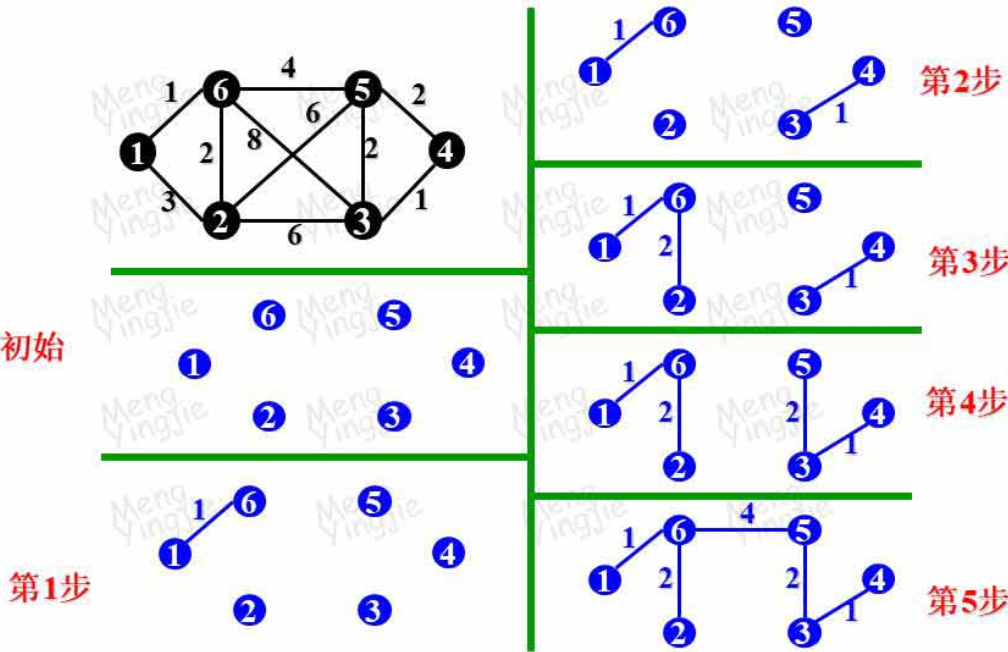
\includegraphics[width=0.7\textwidth]{8.12.png}
    \caption{克鲁斯卡尔(Kruskal)例子}
    \label{fig_install_texlive}
\end{figure}

	\section{有向无环图及应用}
一个无环的有向图,我们称为有向无环图(DAG, directed acyclic graph)。这一节只讨论DAG。是介于树形结构和有向图之间的一种模型,在实际工程应用中价值比较高。
		\subsection{拓扑排序}
			\subsubsection{相关术语}
\begin{itemize}
	\item AOV-网

若有向图G中,顶点表示活动或任务,有向边表示活动或任务之间的优先关系,则此有向图称为顶点表示活动的网络。(AOV-网,Activity On Vertex Network)

一个AOV-网要能够表达一个可执行的工程则其优先关系应当是非自反的。

若存在回路,则说明某项活动的能否进行是要以自身任务的完成作为先决条件。对一个程序来说相当于出现了死循环。因此给定一个AOV-网,当要检测该网所表示的工程是否可以实现时,就可以通过检查其是否有回路来完成。一种有效的方法就是拓扑排序(寻找图的偏序序列的过程)。
	\item 拓扑序列

对于有向图G=(V,E),V中的顶点的线性序列($v_{i1}$, $v_{i2}$, … , $v_{in}$),称作一个拓扑序列,若此结点序列满足如下条件:在G中从顶点u到顶点v有一条路径,则在序列中u必在v之前。

拓扑序列不唯一

任何无环的有向图,其顶点都可以排在一个拓扑序列中

	\item 拓扑排序

寻找图的拓扑序列的过程。
图中的拓扑序列往往不止一个。拓扑排序只需要找到一个。
\end{itemize}

			\subsubsection{拓扑排序基本思想}
\begin{enumerate}
	\item 从图中选择一个入度为零的顶点
	\item 输出该顶点,从图中删除此顶点及其所有的出边
\end{enumerate}
反复执行以上两步,直到所有顶点都输出,此时拓扑排序完成;或者直到剩下的图中再无入度为零的顶点,此时说明图G是有环的图,拓扑排序无法完成。
\begin{figure}[H]
    \centering
    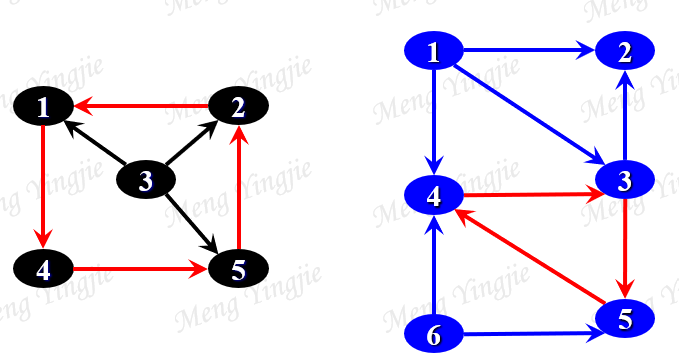
\includegraphics[width=0.7\textwidth]{8.13.png}
    \caption{死锁实例}
    \label{fig_install_texlive}
\end{figure}
			\subsubsection{拓扑排序实现——基于邻接矩阵}
基于基本思想中的关键两步,进行具体细化:
				\begin{enumerate}
					\item 选择入度为零的结点u——选择全零的列u。(行发出,列接收)
					\item 输出顶点,删除出边
						\begin{enumerate}
							\item 顶点的输出
				
				策略:拓扑序列可通过辅助辅助数组S[1..n]保存, 具体取值:
				\begin{figure}[H]
				    \centering
				    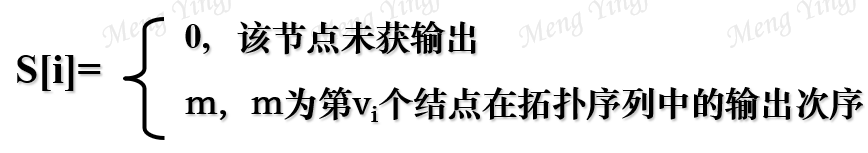
\includegraphics[width=0.7\textwidth]{8.14.png}
				    
				    \label{fig_install_texlive}
				\end{figure}
				
							\item 删除出边,删除u所有出边
				
				删除u所有出边即讲邻接矩阵中第u行置零。
						\end{enumerate}
				\end{enumerate}
算法步骤:
\begin{enumerate}
	\item 辅助数组S置零,输出次序计数器置初值(即:设定顶点的输出的顺序编号的起步值)
	\item 寻找没有输出编号的全零的列u,如果没有,则算法终止。此时S中所有元素都有输出编号,则拓扑排序完成;否则有环。
	\item 将输出次序号赋给S[u]。
	\item 把第u行置成全零。
	\item 输出次序号加1,回到2。

\end{enumerate}
算法复杂度为O(n3)
			\subsubsection{拓扑排序实现——基于邻接表}
\begin{itemize}
	\item 预处理工作
				\begin{itemize}
					\item 存储结构的优化
				
				要获取入度,需有逆邻接表。要删除所有出边,需有邻接表。两个需求无法同时满足。于是做以下处理:选择邻接表,在图建立的时候加一个入度项,计算每个结点的入度。
				\begin{figure}[H]
				    \centering
				    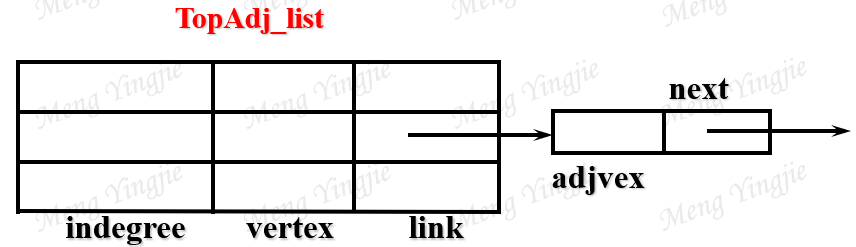
\includegraphics[width=0.7\textwidth]{8.15.png}
				    \caption{邻接表结构设计}
				    \label{fig_install_texlive}
				\end{figure}
				
					\item 设置一个集合存放参与运算的结点
				
				需要一个结构(S)保存其它入度为零的顶点,以备选用。S可以采用栈。
				\end{itemize}
	\item 运算的步骤
		\begin{enumerate}
			\item 搜索邻接表中入度为零的顶点,并令其进栈
			\item 当栈非空时,进行拓扑排序:
				\begin{enumerate}
					\item 退栈,输出栈顶元素u
					\item (循环)在邻接表中扫描u的直接后继顶点k
						\begin{itemize}
							\item 将k入度减一
							\item 若此时k的入度为零,则k入栈
						\end{itemize}
				\end{enumerate}
			\item 若栈空,输出元素不足n则有环,否则拓扑排序完成
		\end{enumerate}
	\item 栈结构的优化设计

为了保存待输出的入度为零的结点(可保存在栈S中),但这需要额外的空间。

邻接表中的入度域是要参与运算的(减法),因此在拓扑排序后,该域将失去实际意义;另外入度为0的顶点的入度域是不会参与运算的,因此,S可借用这些单元作为栈的存储空间;这样可以将入度为零的顶点的入度域组织成一个静态的链栈。此时indegree域相当于next域的作用。
\end{itemize}
		\subsection{关键路径}
			\subsubsection{AOE-网及关注的问题}
与AOV-网对应的是AOE网。AOE-网在企业管理、工程计划等当中有广泛的应用。

若在带权有向图中顶点表示事件,有向边表示活动,权表示活动持续的时间,则此有向图称为边表示活动的网络(AOE-网, Activity On Edge Network).

表示实际工程(或计划)的AOE-网,应该是无环的,且存在唯一入度为零的起始顶点(始点),以及唯一的出度为零的完成顶点(终点)。

关注的点:
\begin{itemize}
	\item 利用事件AOE-网可以进行工程安排估算,研究完成整个工程至少需要多少时间
	\item 为缩短整个工程的完成时间,应该加快哪些活动的速度
\end{itemize}


在AOE-网要解决这些问题,可以采用多种技术:
\begin{itemize}
	\item PERT(Program Evaluation and Re$v_{i}$ew Technique)(程序评价和审定技术)
	\item CPM(Critical Path Method)(关键路径法)
	\item RAMPS(Resources Allocation and Multi-Project Scheduling )(资源分配和多项目调度)

\end{itemize}

	\section{最短路径}
		\subsection{单源最短路径}
单源最短路径是指从一个顶点到其它各顶点之间的最短路径(single-source shortest path)。

迪杰斯特拉(E.W.Dijkstra)于1959年提出了一个寻找单源最短路径的方法。

其基本思想是,设置一个顶点集合S,并不断地作贪心选择来扩充这个集合。该算法属于算法设计方法中的贪心算法(greedy selector)类——总是作出当前看来最好的选择,通过获取局部最优,最终达到获取整体最优)。

		\subsection{每对顶点的最短路径(all-pairs shortest path)}

\chapter{排序}
	\section{基本概念}
		\subsection{概论}
排序是数据结构运算层面的问题。

排序(sorting)是计算机程序设计中的一种重要的运算,其功能是将一个数据元素的任意序列,按照要求重新排列成按一定规则有序的序列。

排序(又称分类)通常可以理解为:根据与项目中所包含的关键字或信息项的有关规则,对信息项目加以排列整理的动作过程。
		\subsection{相关概念}
			\subsubsection{关键字(key)}
如果数据元素(或结点、记录)中的某个数据项的值可以用它标识一个数据元素,则将该数据项称为关键字。

关键字这一项往往不反应事物的本质。
			\subsubsection{主、次关键字}
\begin{itemize}
	\item 主关键字

可以唯一地标识一个记录的关键字称为主关键字(Major Key、Primary Key),实际应用中关键字不加声明时都指的是主关键字。
        Major key:在一个记录中的最主要的关键字;

        Primary key:在文件组织中,进行大量访问时所用关键字。

	\item 次关键字

次关键字(辅助关键字、Secondary Key):可以识别若干记录的关键字称次关键字。
\end{itemize}
			\subsubsection{排序}
设含有n个记录的集合为R={r1,r2,…,rn},其对应的关键字集合为K={k1,k2,…,kn},给定关系$\alpha$,按照关系$\alpha$针对关键字集合K对R进行运算,使得R有如下序列:(r$\alpha$1, r$\alpha$2 ,…, r$\alpha$n),我们将这个操作过程称为排序。
\begin{figure}[H]
    \centering
    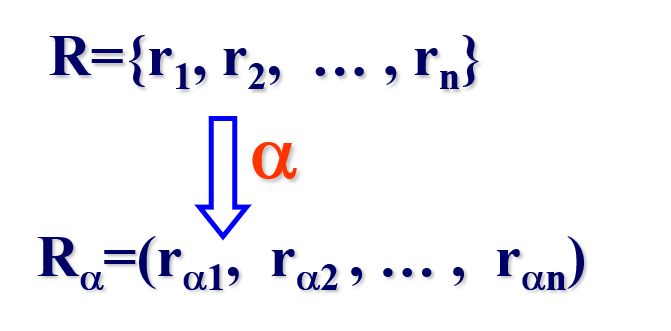
\includegraphics[width=0.7\textwidth]{8.16.png}
    \caption{排序的本质}
    \label{fig_install_texlive}
\end{figure}
本质是在关系$\alpha$下寻找R的一种排列的过程。


			\subsubsection{排序的稳定性}
      在排序关系下,假设排序前ri在rj之前,排序之后领先关系不变,则称此排序过程和排序方法是稳定的,否则是不稳定的。
\begin{figure}[H]
    \centering
    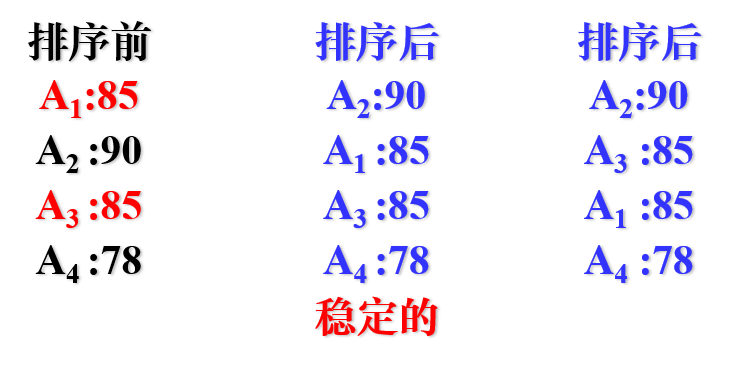
\includegraphics[width=0.7\textwidth]{8.17.png}
    \caption{排序的稳定性例子}
    \label{fig_install_texlive}
\end{figure}
			\subsubsection{排序的分类}
排序一般涉及大量数据,而大规模数据一般都存放于外部存储器上,并以文件的形式出现。因此,依据排序过程中数据所处位置,可以将排序分为两大类:
\begin{itemize}
	\item 内(部)排序:

将整个待排序的文件装入内存,并在其中进行排序,这种排序过程称为内(部)排序(internal sorting)。
	\item 外(部)排序:

由于数据规模过大,排序过程不能在内存中一次完成,需要不断进行内外存数据交换才能完成排序,这样的排序过程称外(部)排序(external sorting)。

\end{itemize}

			\subsubsection{排序的应用}
\begin{itemize}
	\item 作为检索的辅助手段
	\item 作为数据项匹配的手段
\end{itemize}
			\subsubsection{影响排序的因素}
		\subsection{存储结构设计}
排序运算可以遵循前面运用的一些存储结构,但有时为了保证高效的排序,可能还需要设计一些特殊的存储方式。

排序常用的存储结构有以下几种:

			\subsubsection{向量}
待排序的初始文件各记录依其自然顺序存放在连续的一块地址空间中。
			\subsubsection{链表结构}
记录以结点形式按记录原始次序链接起来。

			\subsubsection{地址向量结构}
将要排序文件的各个记录存储到内存的各个块中,这些块的地址一般是不连续的。按各记录的原始次序,将这些的块的首地址依次存入内存的一块连续单元中,由各块的首地址组成了一个向量——地址向量。

这样可实现局部连续,整体不连续的组织模式,这种组织方式具有较高的实用性。

就是原来的索引结构
	\section{插入排序}
		\subsection{插入类排序基本方法}
			\subsubsection{基本思想:}

\begin{enumerate}
	\item 每次只考虑一个待排记录 r
	\item 将 r 按照排序关系插入到一个已经有序的文件适当位置
	\item 重复上述过程直到全部记录插完为止
\end{enumerate}
		\subsection{直接插入排序(straight insertion sort)}
\begin{enumerate}
	\item 将要排序的源文件F=R1,R2,…,Rn,视为两部分:

​ F'=R1; F''= R2,…,Rn
	\item 对F'和F''重复如下工作:
\begin{enumerate}
	\item 从F''中取出一个记录Ri,并将Ri从F''中删除
	\item 将Ri插入到F'并使F'线性有序
\end{enumerate}

\end{enumerate}
第i个记录的插入过程:
\begin{enumerate}
	\item 进行插入准备:先取出第i个元素放入x临时存储(x ← R[i]; j←i-1)
\begin{figure}[H]
    \centering
    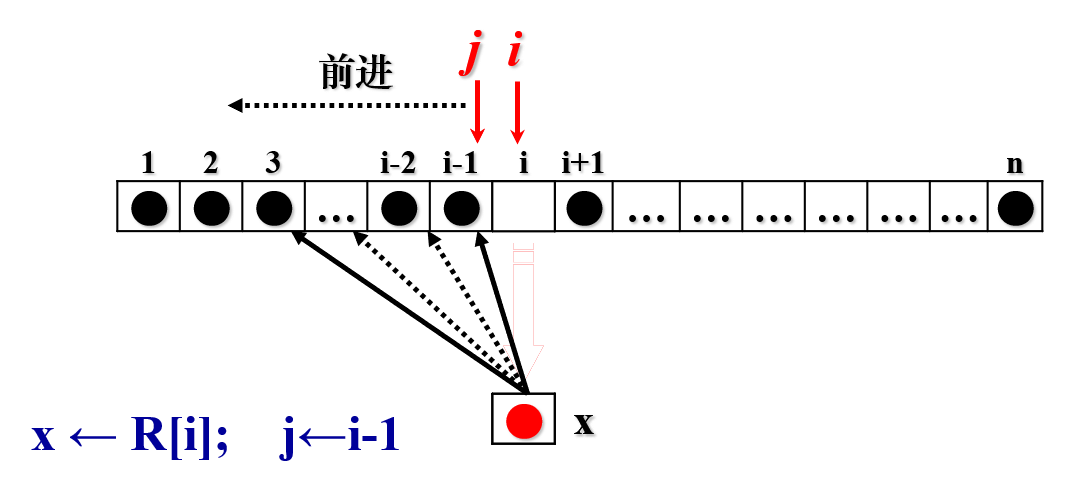
\includegraphics[width=0.7\textwidth]{8.18.png}
    \caption{将第i个元素放入x临时存储}
    \label{fig_install_texlive}
\end{figure}

	\item 寻找插入位置:向前进行比较, 条件:(x.key<R[j].key) and (1 $\le$ j)

	\item 插入元素归位:R[j+1] ← x
\end{enumerate}

\begin{figure}[H]
    \centering
    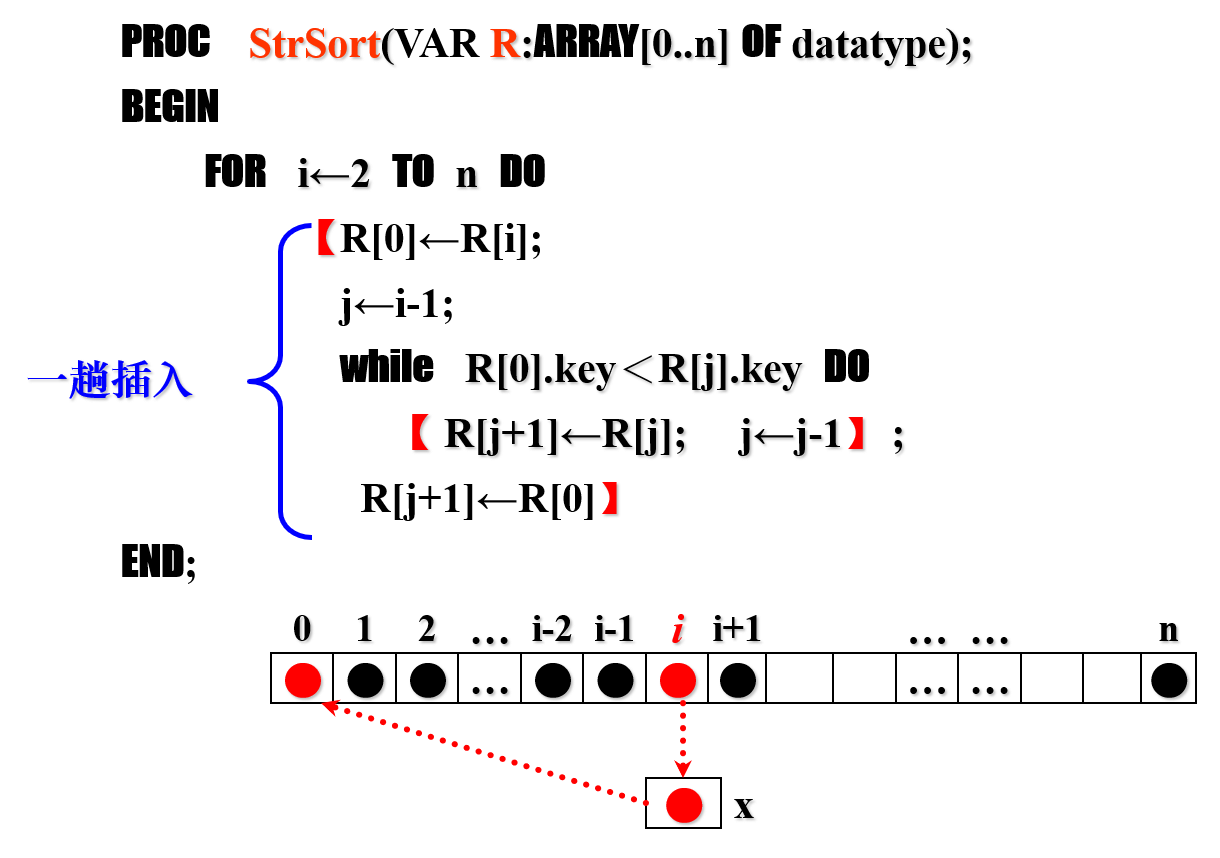
\includegraphics[width=0.7\textwidth]{8.19.png}
    \caption{直接插入算法过程}
    \label{fig_install_texlive}
\end{figure}

		\subsection{二分插入排序(dichotomising  insertion sort)}
也称折半插入排序。与直接插入排序的区别:在插入第i个时搜索采用二分策略。

仅对比较次数有改善,移动次数无影响。算法过程如下:
\begin{figure}[H]
    \centering
    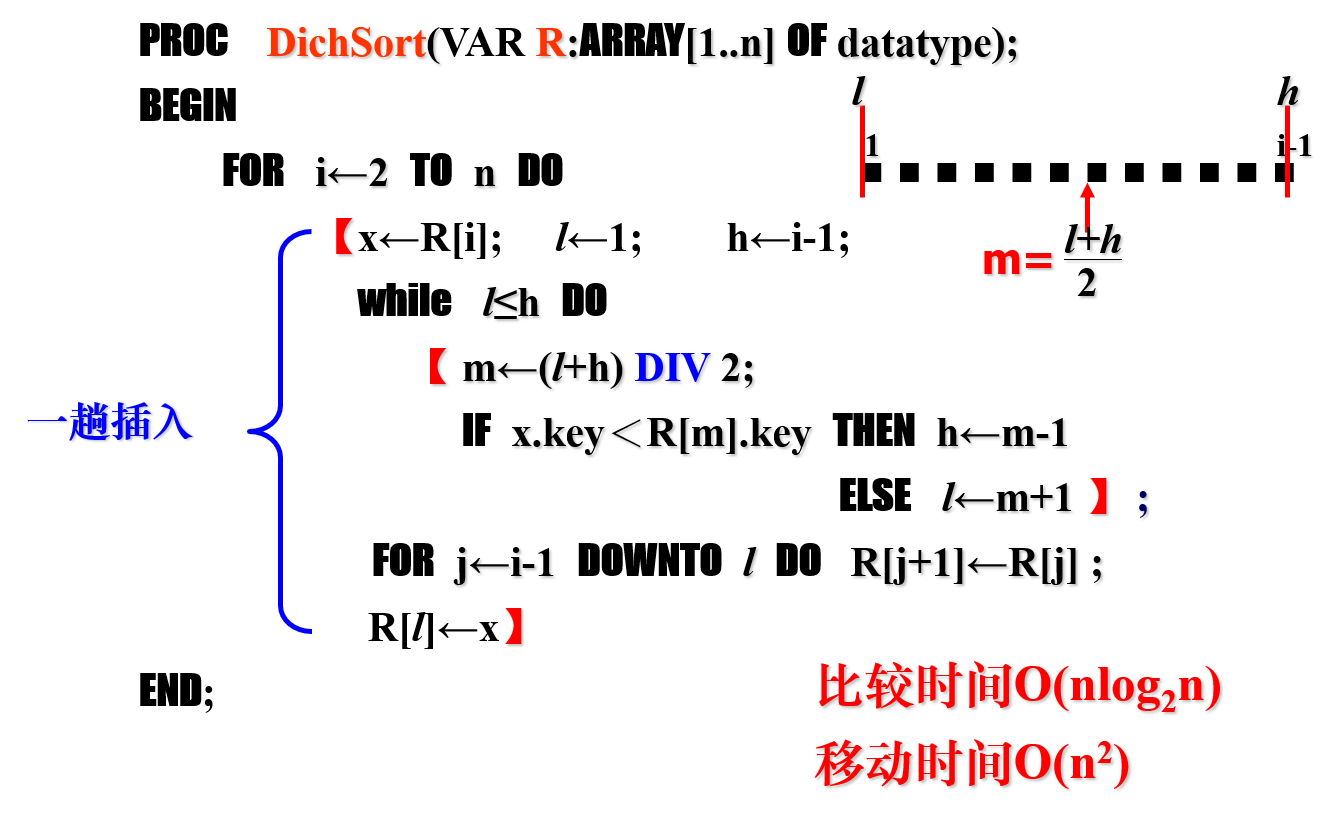
\includegraphics[width=0.7\textwidth]{8.20.png}
    \caption{二分插入算法过程}
    \label{fig_install_texlive}
\end{figure}

		\subsection{2-路插入排序}
在二分插入排序的基础上再改进。

目的:减少排序过程中记录的移动次数。

借助辅助空间D[1..n]。

		\subsection{表插入排序(list inserting sort)}
采用链式结构来组织待排序的数据元素。        

是一种较为古典的算法,仅适用于链结构,下完成分类。

其独到之处是利用链结构的特点,通过变更记录指针来调整记录的逻辑顺序,从而在不发生记录迁移的情况下完成分类。
		\subsection{希尔排序(Shell  sort)}
         又称缩小增量法(diminishing increment sort),是一种快速的排序方法,1959年由D.L.Shell提出。
			\subsubsection{基本思想}
	把对源文件F的排序分成多步来完成,算法在每步中取一个步长 d,将F逻辑上看成 d 个文件。
\begin{enumerate}
	\item 按照插入排序的办法把这 d 个文件分别排序;
	\item 然后缩小 d 
	\item 重复1-2,直到 d=1 的一次排序为止
\end{enumerate}
	\section{交换排序}
		\subsection{交换类排序基本方法}
			\subsubsection{基本思想:}
每次考虑两个待排序的记录。

依据排序关系两两比较待排序记录,并交换不满足顺序要求的那些偶对,直到全部满足为止。

		\subsection{起泡排序(bubble sort)}
			\subsubsection{基本思想:}
先比较R1与R2,如果R1大,则交换R1和R2;然后对R2和R3做同样的处理,重复此过程直到处理完Rn-1和Rn的比较和交换。

这样从(R1, R2), (R2, R3),直到 (Rn-1, Rn)的n-1次比较和交换过程我们称为一趟起泡。

一趟起泡的明显结果是将最大的传到了最后(最终位置)。

显然,第二趟起泡只需进行(R1, R2), (R2, R3),…,(Rn-2, Rn-1)的比较和交换。

这样最多做n-1次起泡即可得到最终有序序列。

若一趟起泡中没有发现元素交换,则已经有序,可以直接终止交换。

			\subsubsection{分析}
\begin{itemize}
	\item 算法是稳定的;      
	\item 算法时间复杂性分析:
\begin{figure}[H]
    \centering
    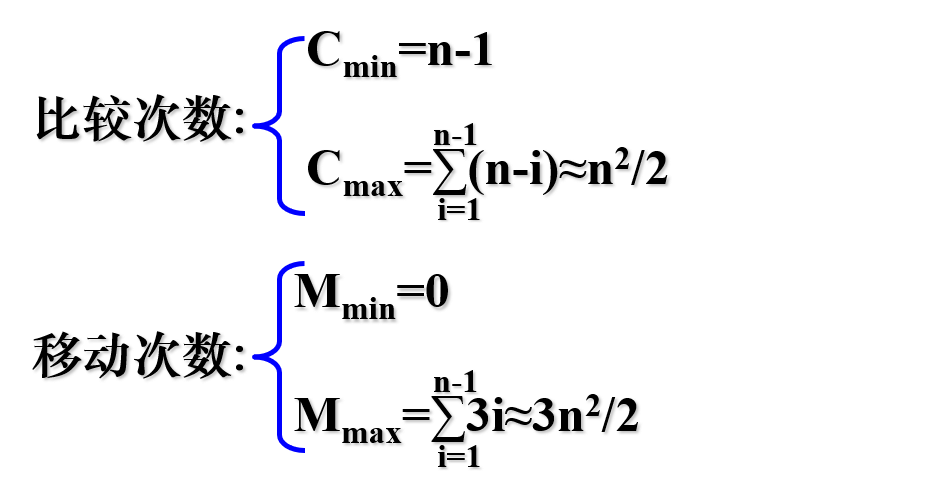
\includegraphics[width=0.7\textwidth]{8.21.png}

\end{figure}
	\item 算法空间复杂性分析:O(1)
\end{itemize}
		\subsection{快速排序(quick sort)}
			\subsubsection{概述}
        也称分区交换排序,或Hoare排序。1962年首先由霍尔(C.A.R.Hoare)提出。
是至今为止内部(比较)排序中较快的一种。它有广泛的应用,典型的应用是UNIX系统调用库函数例程中的qsort函数。
       但快速排序往往由于最差时间代价的性能而在某些应用中无法采用。越接近有序性能越差。
        主要特点是采取了分治的思想。
			\subsubsection{快排基本思想:}
(以下比较指关键的比较,关键字指排序关键字)
\begin{enumerate}
	\item 在待排序的n个记录中任取一个记录r(例如就取第1个),作为轴心元素
	\item 以r为标准将所有记录分为两组。第1组中各记录的关键字都小于r的关键字;第2组中各记录的关键字都大于r的关键字
	\item 并把r排在这两组中间(最终位置),这一过程称为一趟快排
	\item 然后对这两组分别重复上述方法,直到所有记录都排在应有位置上
\end{enumerate}         
			\subsubsection{一趟快排描述}
初始准备:
\begin{itemize}
	\item 建一个额外空间x存放取出来的任意元素
	\item 设置两个指针i,j
\end{itemize}
\begin{figure}[H]
    \centering
    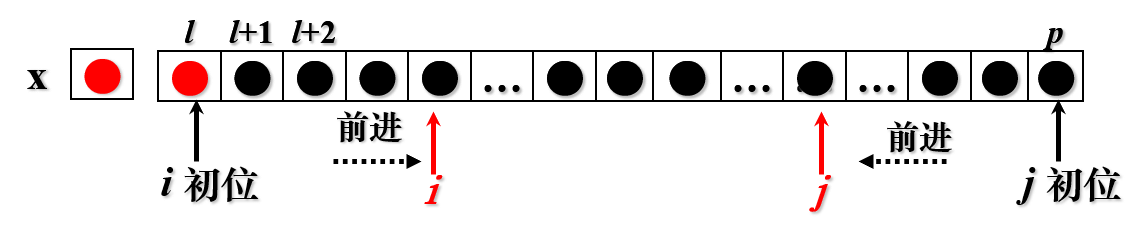
\includegraphics[width=0.7\textwidth]{8.22.png}
    \caption{初始准备}
    \label{fig_install_texlive}
\end{figure}
处理:
\begin{enumerate}
	\item 当(i<j)且R[j].key>x.key时,j指针前进
	\item 如果i<j,则:
\begin{enumerate}
	\item R[j]$\Rightarrow$R[i];  i+1$\Rightarrow$i
	\item 当(i<j)且R[i].key<x.key时,i指针前进
	\item 如果 i<j ,则:R[i]$\Rightarrow$R[j];  j-1$\Rightarrow$j
\end{enumerate}
	\item 如果  i=j ,则本趟结束,否则转⑴
	\item 以上结束后:x$\Rightarrow$ R[i]
\end{enumerate}
			\subsubsection{快排算法过程}

	\section{选择排序}
	\section{合并排序}
	\section{枚举排序}
	\section{分配排序}

\chapter{数据检索}
	\section{基本概念}
		\subsection{概论}
本章集中讨论非数值程序设计中的另一个重要的技术问题——检索 (search,或称为查找seek).
		\subsection{相关概念}
			\subsubsection{检索}
在给定数据结构中查找满足某种条件的数据元素(或结点、记录)的过程。

			\subsubsection{检索的分类}
\begin{itemize}
	\item 基于关键字的检索

在给定的结构中找出关键字等于指定值的结点。检索成功时,往往只得到一个结点即可
	\item 基于属性的检索

在给定结构中找出某属性值等于指定值的结点。检索成功时,检索结果往往是一批结点

\end{itemize}

			\subsubsection{检索方法的分类}
根据检索对象的组织关系和检索对象的存储组织模式,检索算法有三类:
\begin{itemize}
	\item 顺序表和线性表方法
	\item 直接访问法(散列方法);
	\item 树索引方法;


\end{itemize}
			\subsubsection{检索算法的特性}
\begin{itemize}
	\item 内外有别

分内检索和外检索。内检索是内存能够容纳全部记录的情形。 
	\item 静态动态

      静态检索时,表的内容不变(即一个单纯的查找过程);动态检索时,表中的内容不断地在变动(即表有频繁地插入/删除记录的操作)。
	\item 原字变字
s
      原字系指用原来的关键字;所谓变字是指使用经过变换过的关键字。

	\item 数字文字

       指比较时用不用数字的性质。用数字的性质就是象排序算法中那样作各位数的分布计数,而不是直接对关键字进行比较,例如字符树就是使用数字性质。

\end{itemize}

			\subsubsection{检索算法效率的度量}
平均检索长度(ASL, Average Search Length):检索过程中对关键字(或属性)要执行的平均运算次数。
\begin{figure}[H]
    \centering
    
\includegraphics[width=0.7\textwidth]{8.23.png}

\end{figure}
这里的运算在大多数情况下是关键字的比较运算。Pi一般认为是等概率的(即Pi=1/n)
			\subsubsection{相关概念}
	\section{线性表的检索}
		\subsection{概论}
		\subsection{顺序检索}

			\subsubsection{检索方法}
用给定的关键字值与线性表中各结点的相应关键字值进行逐一比较。

找到相等的则检索成功,否则检索失败。

这种方法对顺序分配或链接分配都是适应的。该方法对于待检索文件的结点无排序要求。
			\subsubsection{向量存储时的算法}
			\subsubsection{简单分析}
设每个记录检索概率相等。

检索成功的比较次数:$\mathrm{ASL}=\sum_{i=1}^{n} \frac{i}{n}=\frac{n+1}{2}$

检索不成功的比较次数:n+1.

时间复杂度:O(n)

空间复杂度:O(1)

算法优点:简单易行。

缺点:检索时间长,检索长度与表中结点数成正比。

		\subsection{二分检索}
			\subsubsection{检索方法}
			\subsubsection{二分检索的基本作法}
此方法是将要检索的对象分成两部分,舍弃不包含所需要项目的那一部分,对剩下的部分再用相同的方法进行划分,直到找到所需要的项目或划分部分为空为止。也称对分检索、折半检索。
			\subsubsection{算法过程}
			\subsubsection{简单分析}
设每个记录检索概率相等。

平均检索长度:$\mathrm{ASL}\frac{n+1}{n} \log _{2}(n+1)-1$

n较大时,$\mathrm{ASL}=\log _{2} \mathrm{n}$

为换取快速检索所付出的代价是要将线性表排序;适应于一旦建立起来就很少改动而又需要经常检索的线性表。
			\subsubsection{有序表的其它检索方法}
\begin{itemize}
	\item 斐波那契(Fibonacci)检索
	\item 插值检索
\end{itemize}
		\subsection{分块检索}
既有较快的速度,又能够动态变化——比较实用
			\subsubsection{分块的组织}
分块检索要求把线性表分成若干块,在每一块中记录的存放是任意的,但是块与块之间必须有序.
	

	\section{树形结构的检索}
		\subsection{概论}
		树形结构的一个重要应用就是用来组织目录和符号表。

		树形结构的检索就是针对树目录和树表所组织的检索。

		以树形结构组织的目录我们称为树目录;以树形结构组织的符号表我们称为树表。
		 \subsection{二叉排序树} 
		 二叉检索树的检索效率取决于该二叉树的深度,但该二叉树是动态生成的,由于输入的结点次序的不同可能导致出现不同的二叉树,也可能出现歪树,使其检索性能退化到与顺序检索等同的情况。
		 优势:
		 \begin{itemize}
			\item 性能好
			\item 保证动态有序性
		\end{itemize}
		\subsection{AVL树} 
		这种二叉树它的子树的深度是平衡的,称为平衡二叉树(即AVL-树,或称为均高二叉树)。
		
		按照这种平衡结构构造的二叉树称为最佳二叉排序树或最优二叉排序树。

			\subsubsection{概念} 
				\begin{itemize}
					\item 结点的平衡因子:
					
					结点的左子树高度减去右子树的高度的差值。
					\item AVL-树:
						\begin{itemize}
							\item 一棵空二叉树是AVL-树
							\item 若T是一棵非空二叉树, 其任何结点的左、右子树的高度相差不超过1,则T是AVL-树
						\end{itemize}
				\end{itemize}			
			\subsubsection{AVL-树平衡的保持} 
			在平衡的二叉树中若进行插入或删除将可能导致不平衡情况的出现,这时就要运用一定的规则进行调整。
			\begin{itemize}
				\item 平衡规则
				
				选择离插入(或删除)结点最近的不平衡结点(其平衡因子为±2)开始调整。
				\item 平衡类型
					\begin{itemize}
						\item LL型: 新结点插在 A 的 左子树的 左子树中导致不平衡
						\item RR型: 新结点插在 A 的 右子树的 右子树中导致不平衡
						\item LR型: 新结点插在 A 的 左子树的 右子树中导致不平衡
						\item RL型: 新结点插在 A 的 右子树的 左子树中导致不平衡
					\end{itemize}
			\end{itemize}		
			\subsubsection{调整过程} 
			\begin{itemize}
				\item LL型:
				\begin{figure}[H]
					\centering
					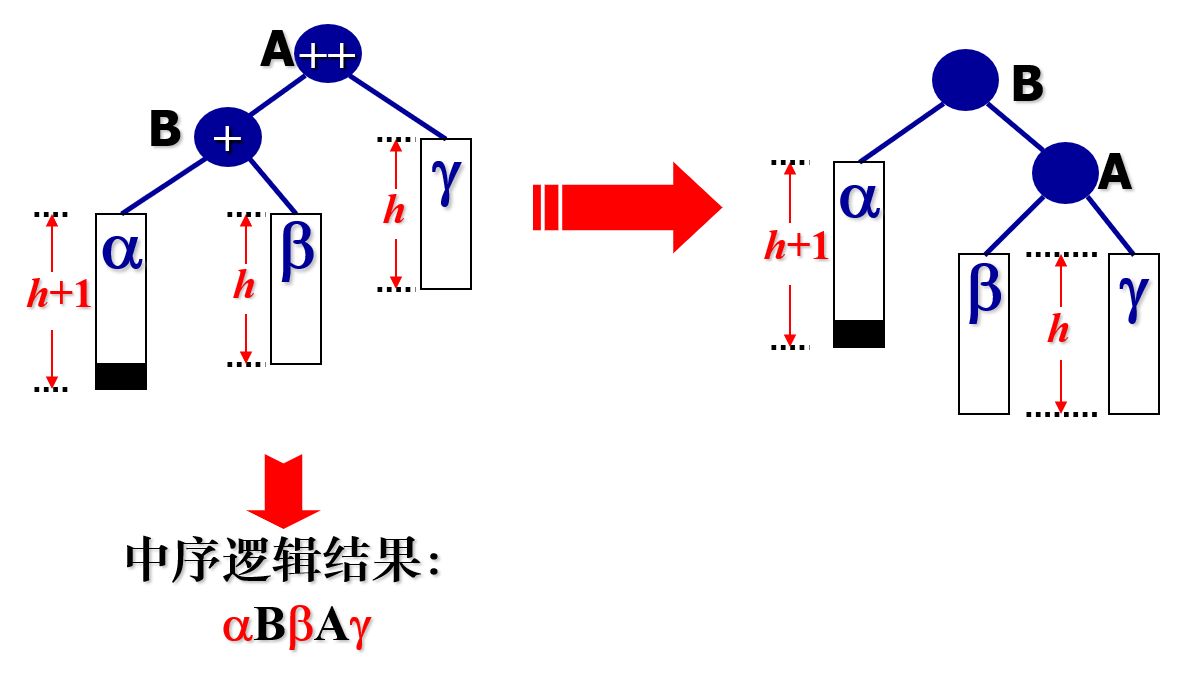
\includegraphics[width=0.7\textwidth]{10.1.png}
					\label{fig_install_texlive}
				\end{figure}			
				\item RR型:
				\begin{figure}[H]
					\centering
					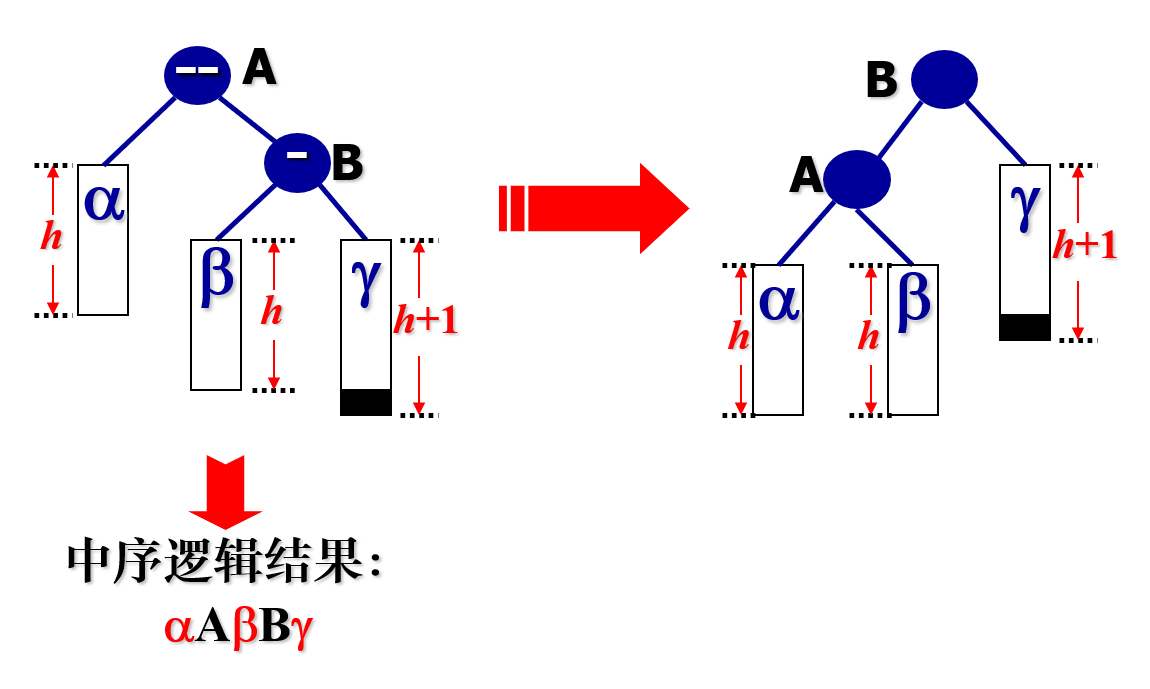
\includegraphics[width=0.7\textwidth]{10.2.png}
					\label{fig_install_texlive}
				\end{figure}	
				\item LR型:
				\begin{figure}[H]
					\centering
					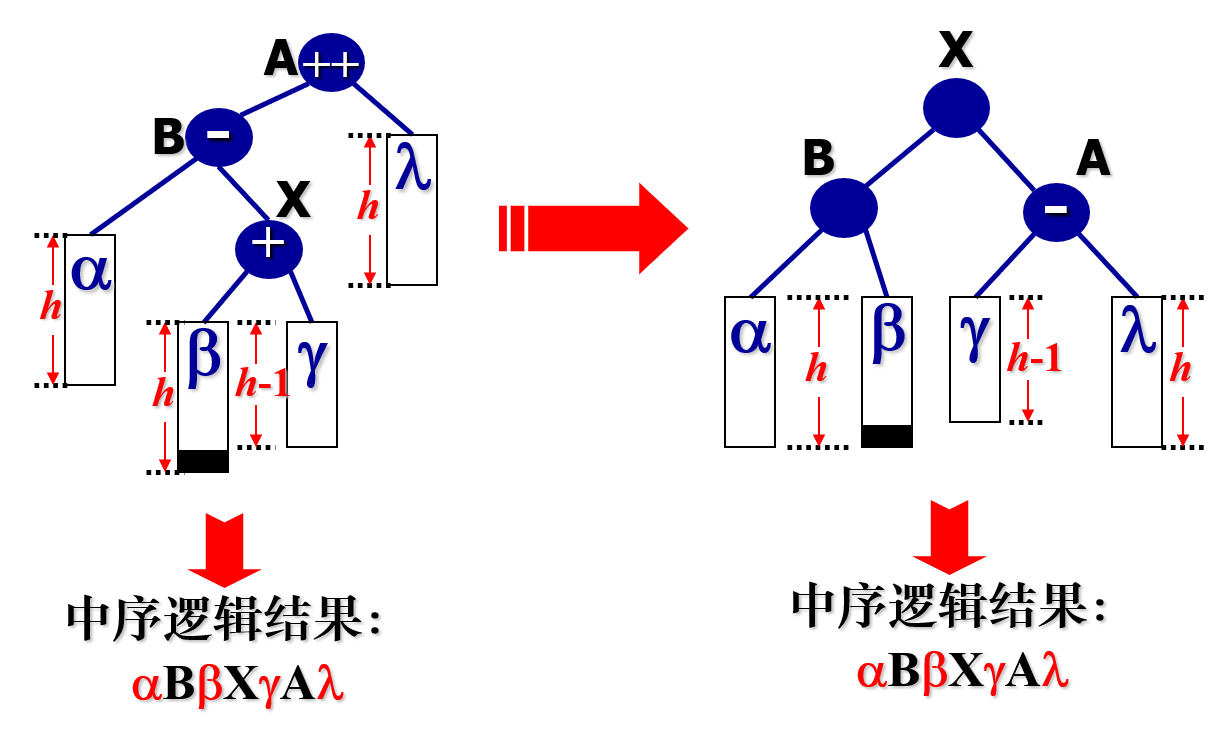
\includegraphics[width=0.7\textwidth]{10.3.png}
					\label{fig_install_texlive}
				\end{figure}	
				\item RL型:
				\begin{figure}[H]
					\centering
					\includegraphics[width=0.7\textwidth]{10.4.png}
					\label{fig_install_texlive}
				\end{figure}	
			\end{itemize}
			总结得:
			\begin{figure}[H]
				\centering
				\includegraphics[width=0.7\textwidth]{10.5.png}
				\label{fig_install_texlive}
			\end{figure}	


	\section{散列表的检索}
		\subsection{概论}
		既是存储方法,也是检索方法。
			\subsubsection{基本思想}
			将关键字看成一个变量,通过一定的函数关系,将函数值解释为存储地址,将结点存入这样计算得到的地址单元中,检索的过程是存储过程的逆过程。

			也称关键字——地址转换法,或关键转换法。

			在散列法中把地址映射函数称为散列函数(hash function)。

			把用散列法组织存储的线性表称为散列表(hash table)。
			\subsubsection{散列函数}
			
		\section{基于属性的检索}

















\chapter{latex部分用法简介}

注意啊,看这个教程,template.pdf配合template.tex\textbf{一起看},才能学习latex怎么用的

网页跳转怎么用?图片插入怎么用?图片横着两个并排站呢?代码怎么插入?表格听说挺复杂?公式听说也挺难的

啥啥啥,你说你还不知道什么是LaTeX ,你去分不清XeLaTex、pdfLaTex,百度一下竟然还让我安装TexLive,这也就算了,甚至还有人说vscode?sublime text3?texstudio?Texmaker?我只是想写个论文排版方便一些,你要干嘛?

上面这些问题,后面都会一点点介绍

\section{用latex需要安装什么}
需要安装texlive,外加一个IDE

\subsection{texlive下载安装}
最近可能出了2020了,可以用兰大的镜像下载应该在用校园网时快一些,额,你还是用清华的镜像吧,我刚才找了一下,兰大镜像这会儿竟然挂了。。。

下载地址\footnote{这个地址会自动更新比如2020版出了以后你下载的就是2020了}: 点下面的字跳转浏览器下载了,方便吧

\begin{itemize}
	\item \href{https://mirrors.tuna.tsinghua.edu.cn/CTAN/systems/texlive/Images/texlive.iso}{TexLive2019 \quad Windows版}
	\item \href{http://tug.org/cgi-bin/mactex-download/MacTeX.pkg}{TexLive2019 \quad Mac版}
\end{itemize}

上面的文件直接双击安装一路next就行,但是texlive这是个啥?

用过python吧,texlive就相当于你下载的python安装包,但是你总不能在终端里写代码吧,一般用pycharm,这个就是IDE,所以你需要再安装一个IDE。


为什么没linux版?用的人不多,真心不想给。。。其实安装文件就是windows的那个版本

\subsubsection{linux系统图形界面安装texlive} % (fold)
\label{ssub:linux图形界面安装方式}

\begin{itemize}
	\item[1. ] 安装per组件: sudo apt-get install perl-tk
	\item[2. ] 加载该ISO文件:sudo mount -o loop texlive2019.iso /mnt (换掉文件路径即可)\footnote{注意:使用该命令会出现错误提示,mount: /dev/loop1 is write-protected, mounting read-only.不必管它}
	\item[3. ]启动图形化安装界面: cd /mnt \& sudo ./install-tl -gui
\end{itemize}

注意倒数第二项,改成 是,创建符号链接,下面那个图是网上随便找的,都差不多

\begin{figure}[H]
    \centering
    \includegraphics[width=0.7\textwidth]{figures/install_texlive.png}

\end{figure}



% subsubsection linux图形界面安装方式 (end)


\subsection{安装IDE} % (fold)
\label{sub:安装ide}

在这之前,请测试texlive是否安装成功!!!在命令行输入tex,显示类似如下结果,注意必须包含“TeX Live 2020”字样

\begin{lstlisting}[language=bash]
    This is TeX, Version 3.14159265 (TeX Live 2020) (preloaded format=tex)
    **
\end{lstlisting}


如果确实安装了,但是没有显示,请根据各自系统自行百度配环境变量,此处不再详细介绍


IDE这个就是写论文的地方,它会调用你刚才安装的texlive,具体用什么,各有所爱,我喜欢sublime text3,这个颜值是真的高,而且体积小,启动快,可以预览公式什么的,很多常用的代码可以自动提示补全,但是这个需要安装插件LaTexTools,pdf需要安装其他的东西进行正反向跳转\footnote{就是点tex文件某一行跳转到pdf对应的地方,点击pdf跳转到tex对应的那一行,mac上安装skim,windows安装sumatra},小白的话就算了吧,想折腾,百度一下吧


另外一个我比较喜欢的是vscode,也需要安装插件,很方便,和sublime text3差不多,但是用起来简单一些,也自己百度去吧

另外几个是\href{https://www.xm1math.net/texmaker}{Texmaker}、或者\href{http://texstudio.sourceforge.net/}{texstudio}\footnote{这个有可能需要番羽墙才能访问,什么意思,别问我,我不知道,啥都不知道},这两个你点名字就跳转官网了,这两个基本上是打开就可可以用,怎么用,自己百度吧,很多详细的图文教程


\begin{figure}[H]
	\centering
	\subfloat[sublime text3]{
        \includegraphics[width=0.4\textwidth]{figures/sublime.png}
    }\qquad
	\subfloat[vscode]{
        \includegraphics[width=0.4\textwidth]{figures/vscode.png}
    }\\
    \caption{我用的IDE}
    \label{fig_ide}
\end{figure}

这两个IDE真的是特别好用,不要再用TexMake或者TexStudio了,连个自动提示都麻烦,预览也没有,最主要的是太丑了,也不能换主题
% subsection 安装ide (end)



\section{常用的一些东西} % (fold)
\label{sec:常用的一些东西}

用到相关的直接到这里复制,然后修改就行

\subsection{国际三线表格} % (fold)
\label{sub:国际三线表格}

\begin{table}[H]
    \centering
    \caption{二硫化钼纳米管参数}
    \begin{tabular}{cccccc} % 控制表格的格式,可以是l,c,r
    \toprule
    参数& m & n & \tabincell{c}{太长了\\换行一下\\原子数}  & 内径 & 长度\\
    \midrule
    数值 & 15 & 15  & 2880 & 2.3014nm & 9.95nm \\
    \bottomrule
    \end{tabular}
    \label{tbl_mos2_nanotube}
\end{table}

这个注意,有多少列,后面就要有多少个c \footnote{否则会报错:Extra alignment tab has been changed to cr.有什么报错百度一下一般就找到了},这个c表示这一列居中(center),靠左的话:l,右:r;

那个label后面的名字自己取,但是不能有重复,是为了引用,比如这样,表格\ref{tbl_mos2_nanotube},方程、图片也是这样引用的,好处是,中间加一个表格导致这个表格的序号变了也没事,你不用再去修改其他地方的引用

\begin{lstlisting}[language = tex]
\begin{table}[H]
    \centering
    \caption{二硫化钼纳米管参数}
    \begin{tabular}{cccccc} % 控制表格的格式,可以是l,c,r
    \toprule
    参数& m & n & 原子数  & 内径 & 长度\\
    \midrule
    数值 & 15 & 15  & 2880 & 2.3014nm & 9.95nm \\
    \bottomrule
    \end{tabular}
    \label{tbl_mos2_nanotube_2}
\end{table}
\end{lstlisting}

\subsection{换页表格} % (fold)

我是真的没想到有的人表格居然这么长,竟然能有三页。。。。


\begin{longtable}{cccccc} % 控制表格的格式,可以是l,c,r
    \caption{二硫化钼纳米管参数}\label{tbl_mos2_nanotube}\\
    \toprule
    参数& m & n & 原子数 & 内径 & 长度\\
    \midrule
    数值 & 15 & 15  & 2880 & 2.3014nm & 9.95nm \\
    数值1 & 15 & 15  & 2880 & 2.3014nm & 9.95nm \\
    数值2 & 15 & 15  & 2880 & 2.3014nm & 9.95nm \\
    数值3 & 15 & 15  & 2880 & 2.3014nm & 9.95nm \\
    数值4 & 15 & 15  & 2880 & 2.3014nm & 9.95nm \\
    数值5 & 15 & 15  & 2880 & 2.3014nm & 9.95nm \\
    数值6 & 15 & 15  & 2880 & 2.3014nm & 9.95nm \\
    数值7 & 15 & 15  & 2880 & 2.3014nm & 9.95nm \\
    数值8 & 15 & 15  & 2880 & 2.3014nm & 9.95nm \\
    数值9 & 15 & 15  & 2880 & 2.3014nm & 9.95nm \\
    数值10 & 15 & 15  & 2880 & 2.3014nm & 9.95nm \\
    数值11 & 15 & 15  & 2880 & 2.3014nm & 9.95nm \\
    数值12 & 15 & 15  & 2880 & 2.3014nm & 9.95nm \\
    数值13 & 15 & 15  & 2880 & 2.3014nm & 9.95nm \\
    数值14 & 15 & 15  & 2880 & 2.3014nm & 9.95nm \\
    数值15 & 15 & 15  & 2880 & 2.3014nm & 9.95nm \\
    数值16 & 15 & 15  & 2880 & 2.3014nm & 9.95nm \\
    数值17 & 15 & 15  & 2880 & 2.3014nm & 9.95nm \\
    数值18 & 15 & 15  & 2880 & 2.3014nm & 9.95nm \\
    数值19 & 15 & 15  & 2880 & 2.3014nm & 9.95nm \\
    数值20 & 15 & 15  & 2880 & 2.3014nm & 9.95nm \\
    \bottomrule
\end{longtable}

    

% subsection 国际三线表格 (end)


\subsection{字体} % (fold)
\label{sub:字体}

\begin{table}[H]
    \centering
    \caption{字体}
    \begin{tabular}{ccccccc} % 控制表格的格式
    \toprule
    名称& 加粗 & 倾斜 & 宋体  & 仿宋 & 黑体 \\
    \midrule
    显示 & \textbf{兰朵儿} & \textit{兰朵儿}  & \songti{兰朵儿} & \fangsong{兰朵儿} & \heiti{兰朵儿}  \\
    显示 & \textbf{ldr} & \textit{ldr}  & \songti{ldr} & \fangsong{ldr} & \heiti{ldr}  \\
    \bottomrule
    \end{tabular}
    \label{tbl_font}
\end{table}
发现没,中文斜体没有效果的,你可以自定义,这个自己百度吧;而且加粗也windows系统上也是没有效果的,一般都改成了黑体(比如这个模板中成绩页等加粗的地方都是用的黑体),当然你也可以自定义。怎么做,百度吧



% subsection 常用的 (end)

\subsection{公式} % (fold)
\label{sub:公式}
所有的符号都要用美元符号包裹\$,需要用到某一个但是不知道,直接百度,基本上都有
\begin{table}[H]
    \centering
    \caption{公式}
    \begin{tabular}{cccccccccc} % 控制表格的格式
    \toprule
    名称& 分数 & 下角标 & 上角标  & 矢量 & 根号 & 希腊字母 & 点乘 & 叉乘 & 矢量\\
    \midrule
    显示 & $\frac{1}{2}$ & $O_2$  & $a^2$ & $\vec{AB}$ & $\sqrt[2]{3}$ & $\theta$ & $\cdot$ & $\times$& $\vec{a}$\\
   
    \bottomrule
    \end{tabular}
    \label{tbl_gs}
\end{table}

但是有时候我们只是正文中想用$MoS_2$,它竟然斜体,不想斜体,我写了个命令,这样用\eqrm{MoS_2},正的吧,常用的命令可以自定义

% subsection 公式 (end)

\subsection{左边大括号} % (fold)
\label{sub:左边大括号}

\begin{equation}
    \left\{
    \begin{array}{rcl}
        \vec{e_1} &= \frac{3a}{2} \vec{i} + \frac{\sqrt{3a}}{2} \vec{j} \\
        \vec{e_2} &= \frac{3a}{2} \vec{i} - \frac{\sqrt{3a}}{2} \vec{j}
    \end{array}
    \right.
    \label{e1e2}
\end{equation}

注意后面有个方程的编号,如果想取消,把上下的两个$equation$改成$equation*$

\begin{equation*}
    \left\{
    \begin{array}{rcl}
        \vec{e_1} &= \frac{3a}{2} \vec{i} + \frac{\sqrt{3a}}{2} \vec{j} \\
        \vec{e_2} &= \frac{3a}{2} \vec{i} - \frac{\sqrt{3a}}{2} \vec{j}
    \end{array}
    \right.
    \label{e1e2_2}
\end{equation*}

% subsection 左边大括号 (end)

\subsection{复杂公式} % (fold)
\label{sub:复杂公式}
不会输出的符号,请百度,啥都有

\begin{equation}
\hat{H}=\frac{\epsilon}{2}\hat{\sigma}_{z}-\frac{\Delta}{2}\hat{\sigma}_{x}+\sum_{k}\omega_{k}\hat{b}_{k}^{\dagger}\hat{b}_{k}+\sum_{k}\frac{g_{k}}{2}\hat{\sigma}_{z}(\hat{b}_{k}+\hat{b}_{k}^{\dagger})\label{eq:sbm}
\end{equation}

% subsection 复杂公式 (end)


\subsection{等号对齐站} % (fold)
\label{sub:等号对齐站}

主要是用这个aligned放在了方程的环境里,等号前面\&控制对齐,每一行后面双斜杠换行

\begin{equation}
    \begin{aligned}
        \vec{CH} & = m\cdot \vec{e_1} + n\cdot \vec{e_2} \\
        & = \frac{3(m+n)a}{2} \vec{i} + \frac{\sqrt{3}(m-n)a}{2} \vec{j} 
    \end{aligned}
    \label{ch}
\end{equation}

% subsection 等号对齐站 (end)

\subsection{矩阵乘法} % (fold)
\label{sub:矩阵乘法}

其实就是几个array组合

\begin{equation}
    \left[ 
    \begin{array}{c}
    x'\\
    y'\\
    \end{array}
    \right]=
    \left[ 
    \begin{array}{cc}
    cos \theta & sin \theta \\
    - sin \theta & cos \theta 
    \end{array}
    \right]
    \cdot
    \left[ 
    \begin{array}{c}
        x\\
        y\\
    \end{array}
    \right]
\end{equation}
% subsection 矩阵乘法 (end)


\subsection{图,并列排} % (fold)
\label{sub:图_并列排}

这一句代表这个图片宽度为一行文本宽度的$\frac{3}{10}$
\begin{lstlisting}[language = tex]
width=0.3\textwidth
\end{lstlisting}



\begin{figure}[H]
	\centering
	\subfloat[首页]{
        \includegraphics[width=0.3\textwidth]{figures/ldr1.jpg}
    }
	\subfloat[课表]{
        \includegraphics[width=0.3\textwidth]{figures/ldr2.jpg}
    }
	\subfloat[我的]{
        \includegraphics[width=0.3\textwidth]{figures/ldr4.jpg}
    }\\	
    \caption{i兰大易班截图}
    \label{fig_ldr}
\end{figure}

% subsection 图_并列排 (end)


\subsection{附页代码} % (fold)
\label{sub:附页代码}
可以在LZUThesis.clc里面修改代码格式

java代码
\begin{lstlisting}[language = java]
    System.out.print("i兰大易班")
    // 试一下中文注释
\end{lstlisting}


tex代码
\begin{lstlisting}[language = tex]
    width=0.3\textwidth
    % 注释
\end{lstlisting}

python代码
\begin{lstlisting}[language = python]
    print("i兰大易班")
    # 注释
\end{lstlisting}

matlab代码有专门的库,但是没必要高亮太多,而且中文适配有问题,直接按照下面这个就可以
\begin{lstlisting}[language = matlab]
    display("i兰大易班")
    % 注释
\end{lstlisting}

% subsection 附页代码 (end)

\subsection{参考文献} % (fold)
\label{sub:参考文献}

这个,百度学术、谷歌学术等网站都可以导出bibtex格式的参考文献(知网不行,网上有个人写了个转换器,但是windows用不了,就不放了,尽量用谷歌学术把那个文献找出来吧),直接放在bib/database.bib文件里、知网需要用其他东西转换,但是我建议用mendeley这个软件管理文献,然后可以导出bibtex格式的,甚至可以直接复制引用,很方便\cite{partl2016, tenne1992polyhedral, tussyadiah2015hotels}。

有些人希望多个参考文献同时引用时用[1-3]而不是[1,2,3],所以我加了个包cite。(2020-5-18)

具体怎么用可以百度,我这里告诉你什么可以用,但是具体的,建议百度,更靠谱一些。


有参考文献时,编译要经过4步,直接XeLaTeX --> BibTeX --> XeLaTeX --> XeLaTeX,不然很多问题,我用的sublime text3,配合插件LatexTool,直接快快捷键ctrl - B,就可以自动完成4步了,很方便

% subsection 参考文献 (end)

% section 图标等常用的教程 (end)




%论文后部
\backmatter


%=======%
%引入参考文献文件
%=======%
\bibdatabase{bib/database}%bib文件名称 仅修改bib/ 后部分
\printbib
% \nocite{*} %显示数据库中有的,但是正文没有引用的文献



\Appendix


这里是附录页,附上你的程序或必要的相关知识

{\bfseries 编译方式:} XeLaTeX -->BibTeX --> XeLaTeX-->XeLaTeX


\Thanks

感谢蒙老师的教导;感谢物理院余航学长开源的LaTeX模板;感谢我电脑没有在中途死机;感谢我的朋友们。


%=====%
%论文(设计)成绩:注意2007的模板要求,成绩页在最后,2020要求成绩页在摘要前面
%=====%

% 下面这些注释掉可以去掉成绩、评语什么的
\supervisorcomment{}

\recommendedgrade{}

\supervisorsignature{
    \raisebox{-10pt}{
    }
}

\committeecomment{}

\finalgrade{}
% 上面这些注释掉可以去掉成绩、评语什么的

\Grade %这一句才是成绩页,上面是填写


\end{document}